
The results of the search, still blinded are shown in Table~\ref{tab:result}.
The $M_T$ distributions, still blinded, for increasing values of \met\
are shown in Fig~\ref{fig:mtsig1},\ref{fig:mtsig2},\ref{fig:mtsig3}.


	\begin{table}[!h]																															
	\begin{center}																															
	{\footnotesize																															
	\begin{tabular}{l||c|c|c|c|c|c|c}																															
	\hline																															
	Sample		&	SRA			&	SRB			&	SRC			&	SRD			&	SRE			&	SRF			&	SRG\\				
	\hline																															
	\hline																															
	\multicolumn{8}{c}{Muon}	\\																														
	\hline																															
	\ttdl\  		&$	330.6	\pm	21.9	$&$	183.4	\pm	20.7	$&$	59.5	\pm	10.0	$&$	22.5	\pm	6.2	$&$	9.0	\pm	3.9	$&$	3.7	\pm	1.8	$&$	2.2	\pm	1.2	$	\\
	\ttsl\ \& single top (1\Lep) 		&$	92.8	\pm	27.5	$&$	41.0	\pm	8.6	$&$	11.5	\pm	3.5	$&$	7.7	\pm	3.4	$&$	0.7	\pm	0.6	$&$	0.3	\pm	0.2	$&$	0.2	\pm	0.2	$	\\
	\wjets\ 		&$	19.2	\pm	4.5	$&$	10.0	\pm	2.2	$&$	3.1	\pm	1.0	$&$	1.2	\pm	0.6	$&$	0.6	\pm	0.4	$&$	0.4	\pm	0.3	$&$	0.2	\pm	0.2	$	\\
	Rare 		&$	33.2	\pm	16.6	$&$	22.7	\pm	11.4	$&$	9.0	\pm	4.5	$&$	4.8	\pm	2.4	$&$	2.9	\pm	1.5	$&$	1.2	\pm	0.6	$&$	1.0	\pm	0.5	$	\\
	\hline																															
	Total 		&$	475.8	\pm	37.8	$&$	257.2	\pm	24.2	$&$	83.2	\pm	11.3	$&$	36.2	\pm	7.4	$&$	13.3	\pm	4.2	$&$	5.5	\pm	1.9	$&$	3.6	\pm	1.3	$	\\
	\hline																															
	\hline																															
	Data 		&$	?			$&$	?			$&$	?			$&$	?			$&$	?			$&$	?			$&$	?			$	\\
	\hline																															
	\hline																															
	\hline																															
	\multicolumn{8}{c}{Electron}	\\																														
	\hline																															
	\ttdl\  		&$	248.1	\pm	16.9	$&$	144.4	\pm	16.6	$&$	51.1	\pm	8.8	$&$	16.2	\pm	4.6	$&$	5.5	\pm	2.5	$&$	2.5	\pm	1.3	$&$	1.3	\pm	0.7	$	\\
	\ttsl\ \& single top (1\Lep) 		&$	68.0	\pm	20.2	$&$	31.2	\pm	6.6	$&$	9.3	\pm	2.8	$&$	4.9	\pm	2.1	$&$	0.5	\pm	0.4	$&$	0.2	\pm	0.2	$&$	0.2	\pm	0.2	$	\\
	\wjets\ 		&$	14.3	\pm	3.3	$&$	7.5	\pm	1.7	$&$	2.4	\pm	0.8	$&$	0.8	\pm	0.4	$&$	0.4	\pm	0.3	$&$	0.3	\pm	0.2	$&$	0.1	\pm	0.2	$	\\
	Rare 		&$	25.8	\pm	12.9	$&$	15.8	\pm	7.9	$&$	7.1	\pm	3.6	$&$	2.9	\pm	1.5	$&$	0.7	\pm	0.4	$&$	0.3	\pm	0.2	$&$	0.1	\pm	0.1	$	\\
	\hline																															
	Total 		&$	356.2	\pm	28.4	$&$	198.9	\pm	19.0	$&$	69.9	\pm	9.7	$&$	24.7	\pm	5.3	$&$	7.1	\pm	2.5	$&$	3.4	\pm	1.3	$&$	1.7	\pm	0.8	$	\\
	\hline																															
	\hline																															
	Data 		&$	?			$&$	?			$&$	?			$&$	?			$&$	?			$&$	?			$&$	?			$	\\
	\hline																															
	\hline																															
	\hline																															
	\multicolumn{8}{c}{Muon+Electron Combined}		\\																													
	\hline																															
	\ttdl\  		&$	578.7	\pm	38.1	$&$	327.8	\pm	36.6	$&$	110.6	\pm	18.3	$&$	38.7	\pm	10.5	$&$	14.5	\pm	6.2	$&$	6.2	\pm	2.9	$&$	3.5	\pm	1.8	$	\\
	\ttsl\ \& single top (1\Lep) 		&$	160.8	\pm	47.7	$&$	72.2	\pm	15.1	$&$	20.8	\pm	6.3	$&$	12.6	\pm	5.4	$&$	1.2	\pm	0.9	$&$	0.6	\pm	0.4	$&$	0.4	\pm	0.3	$	\\
	\wjets\ 		&$	33.5	\pm	8.0	$&$	17.5	\pm	4.1	$&$	5.5	\pm	1.9	$&$	2.0	\pm	1.2	$&$	1.0	\pm	0.7	$&$	0.7	\pm	0.5	$&$	0.3	\pm	0.4	$	\\
	Rare 		&$	59.0	\pm	29.5	$&$	38.5	\pm	19.3	$&$	16.1	\pm	8.1	$&$	7.7	\pm	3.9	$&$	3.6	\pm	1.8	$&$	1.5	\pm	0.8	$&$	1.1	\pm	0.6	$	\\
	\hline																															
	Total 		&$	832.0	\pm	65.7	$&$	456.1	\pm	42.5	$&$	153.0	\pm	20.6	$&$	60.9	\pm	12.4	$&$	20.3	\pm	6.5	$&$	8.9	\pm	3.0	$&$	5.3	\pm	1.9	$	\\
	\hline																															
	\hline																															
	Data 		&$	?			$&$	?			$&$	?			$&$	?			$&$	?			$&$	?			$&$	?			$	\\
	\hline																															
	\end{tabular}}																															
	\caption{The result of the search.																															
	\label{tab:result}																															
	\end{center}}																															
	\end{table}																															


\begin{table}[!h]																	
\begin{center}																	
{\footnotesize																	
\begin{tabular}{l||c|c|c|c|c|c|c}																	
\hline																	
Sample		&	SRA	&	SRB	&	SRC	&	SRD	&	SRE	&	SRF	&	SRG	\\	
\hline																	
\hline																	
\multicolumn{8}{c}{Muon}	\\																
\hline																	
\wjets\ cross-section		&$	9.0	$&$	6.5	$&$	2.6	$&$	1.2	$&$	0.6	$&$	0.3	$&$	0.2	$	\\
rare cross-sections		&$	10.4	$&$	6.6	$&$	3.0	$&$	1.9	$&$	1.3	$&$	0.5	$&$	0.4	$	\\
top tail-to-peak ratio		&$	67.1	$&$	24.8	$&$	7.6	$&$	2.2	$&$	1.0	$&$	0.5	$&$	0.2	$	\\
\wjets\ tail-to-peak ratio		&$	34.5	$&$	14.9	$&$	5.1	$&$	2.3	$&$	1.3	$&$	0.7	$&$	0.5	$	\\
\ttdl\ (stat)		&$	6.0	$&$	4.4	$&$	2.4	$&$	1.6	$&$	1.0	$&$	0.6	$&$	0.5	$	\\
$K_3$ and $K_4$		&$	9.9	$&$	5.5	$&$	1.8	$&$	0.7	$&$	0.3	$&$	0.1	$&$	0.1	$	\\
2nd lepton veto		&$	6.5	$&$	3.6	$&$	1.2	$&$	0.4	$&$	0.2	$&$	0.1	$&$	0.0	$	\\
\ttdl\ (CR4 and CR5 closure tests)		&$	16.5	$&$	18.3	$&$	8.9	$&$	5.6	$&$	3.6	$&$	1.5	$&$	0.9	$	\\
$M_T$ peak data and MC (stat)		&$	6.0	$&$	6.1	$&$	3.4	$&$	2.0	$&$	1.2	$&$	0.8	$&$	0.8	$	\\
\hline																	
\hline																	
total		&$	79.8	$&$	36.8	$&$	14.2	$&$	7.3	$&$	4.5	$&$	2.1	$&$	1.4	$	\\
\hline																	
\hline																	
\hline																	
\multicolumn{8}{c}{Electron}	\\																
\hline																	
\wjets\ cross-section		&$	6.8	$&$	5.0	$&$	2.2	$&$	1.0	$&$	0.3	$&$	0.2	$&$	0.1	$	\\
rare cross-sections		&$	8.1	$&$	4.6	$&$	2.2	$&$	0.9	$&$	0.1	$&$	0.1	$&$	0.0	$	\\
top tail-to-peak ratio		&$	49.2	$&$	18.9	$&$	6.1	$&$	1.4	$&$	0.7	$&$	0.4	$&$	0.2	$	\\
\wjets\ tail-to-peak ratio		&$	25.3	$&$	11.4	$&$	4.1	$&$	1.4	$&$	0.8	$&$	0.6	$&$	0.5	$	\\
\ttdl\ (stat)		&$	5.2	$&$	3.9	$&$	2.4	$&$	1.3	$&$	0.7	$&$	0.5	$&$	0.3	$	\\
$K_3$ and $K_4$		&$	7.4	$&$	4.3	$&$	1.5	$&$	0.5	$&$	0.2	$&$	0.1	$&$	0.0	$	\\
2nd lepton veto		&$	4.9	$&$	2.9	$&$	1.0	$&$	0.3	$&$	0.1	$&$	0.0	$&$	0.0	$	\\
\ttdl\ (CR4 and CR5 closure tests)		&$	12.4	$&$	14.4	$&$	7.7	$&$	4.0	$&$	2.2	$&$	1.0	$&$	0.5	$	\\
$M_T$ peak data and MC (stat)		&$	5.7	$&$	5.4	$&$	3.2	$&$	1.7	$&$	0.9	$&$	0.6	$&$	0.4	$	\\
\hline																	
\hline																	
total		&$	58.8	$&$	28.5	$&$	11.9	$&$	5.2	$&$	2.7	$&$	1.5	$&$	0.9	$	\\
\hline																	
\hline																	
\hline																	
\multicolumn{8}{c}{Muon+Electron Combined}	\\																
\hline																	
\wjets\ cross-section		&$	15.9	$&$	11.5	$&$	4.8	$&$	2.2	$&$	0.9	$&$	0.4	$&$	0.3	$	\\
rare cross-sections		&$	18.5	$&$	11.1	$&$	5.1	$&$	2.7	$&$	1.4	$&$	0.6	$&$	0.4	$	\\
top tail-to-peak ratio		&$	116.3	$&$	43.6	$&$	13.7	$&$	3.6	$&$	1.7	$&$	1.0	$&$	0.3	$	\\
\wjets\ tail-to-peak ratio		&$	59.8	$&$	26.3	$&$	9.1	$&$	3.7	$&$	2.1	$&$	1.3	$&$	1.0	$	\\
\ttdl\ (stat)		&$	11.2	$&$	8.3	$&$	4.8	$&$	2.9	$&$	1.7	$&$	1.1	$&$	0.8	$	\\
$K_3$ and $K_4$		&$	17.4	$&$	9.8	$&$	3.3	$&$	1.2	$&$	0.4	$&$	0.2	$&$	0.1	$	\\
2nd lepton veto		&$	11.5	$&$	6.5	$&$	2.2	$&$	0.8	$&$	0.3	$&$	0.1	$&$	0.1	$	\\
\ttdl\ (CR4 and CR5 closure tests)		&$	28.9	$&$	32.8	$&$	16.6	$&$	9.7	$&$	5.8	$&$	2.5	$&$	1.4	$	\\
$M_T$ peak data and MC (stat)		&$	8.7	$&$	8.4	$&$	4.7	$&$	2.6	$&$	1.5	$&$	1.0	$&$	0.9	$	\\
\hline																	
\hline																	
total		&$	138.4	$&$	64.8	$&$	25.6	$&$	12.2	$&$	7.0	$&$	3.4	$&$	2.2	$	\\
\hline																	
\end{tabular}}																	
\caption{Contributions to the total uncertainties.}																	
\label{tab:uncertaintycomponents}																	
\end{center}																	
\end{table}																	



\begin{table}[!h]																	
\begin{center}																	
{\footnotesize																	
\begin{tabular}{l||c|c|c|c|c|c|c}																	
\hline																	
Sample		&	SRA	&	SRB	&	SRC	&	SRD	&	SRE	&	SRF	&	SRG	\\	
\hline																	
\hline																	
\multicolumn{8}{c}{Muon}	\\																
\hline																	
\wjets\ cross-section		&$	1.7	\% $&$	2.3	\% $&$	3.0	\% $&$	3.7	\% $&$	4.2	\% $&$	4.2	\% $&$	5.3	\% $	\\
rare cross-sections		&$	2.0	\% $&$	2.3	\% $&$	3.4	\% $&$	5.6	\% $&$	8.8	\% $&$	8.0	\% $&$	10.4	\% $	\\
top tail-to-peak ratio		&$	12.6	\% $&$	8.7	\% $&$	8.6	\% $&$	6.7	\% $&$	7.1	\% $&$	8.6	\% $&$	4.6	\% $	\\
\wjets\ tail-to-peak ratio		&$	6.5	\% $&$	5.3	\% $&$	5.8	\% $&$	6.9	\% $&$	8.9	\% $&$	12.0	\% $&$	13.6	\% $	\\
\ttdl\ (stat)		&$	1.1	\% $&$	1.5	\% $&$	2.8	\% $&$	4.7	\% $&$	6.7	\% $&$	9.7	\% $&$	12.2	\% $	\\
$K_3$ and $K_4$		&$	1.9	\% $&$	1.9	\% $&$	2.0	\% $&$	2.0	\% $&$	1.9	\% $&$	1.8	\% $&$	1.8	\% $	\\
2nd lepton veto		&$	1.2	\% $&$	1.3	\% $&$	1.3	\% $&$	1.3	\% $&$	1.2	\% $&$	1.2	\% $&$	1.2	\% $	\\
\ttdl\ (CR4 and CR5 closure tests)		&$	3.1	\% $&$	6.5	\% $&$	10.2	\% $&$	16.9	\% $&$	25.1	\% $&$	23.8	\% $&$	23.4	\% $	\\
$M_T$ peak data and MC (stat)		&$	1.1	\% $&$	2.1	\% $&$	3.8	\% $&$	6.0	\% $&$	8.6	\% $&$	13.1	\% $&$	20.0	\% $	\\
\hline																	
\hline																	
total		&$	15.0	\% $&$	13.0	\% $&$	16.1	\% $&$	22.1	\% $&$	31.3	\% $&$	33.7	\% $&$	37.9	\% $	\\
\hline																	
\hline																	
\hline																	
\multicolumn{8}{c}{Electron}	\\																
\hline																	
\wjets\ cross-section		&$	1.7	\% $&$	2.3	\% $&$	2.9	\% $&$	4.2	\% $&$	4.4	\% $&$	4.5	\% $&$	4.6	\% $	\\
rare cross-sections		&$	2.1	\% $&$	2.1	\% $&$	2.9	\% $&$	3.7	\% $&$	1.9	\% $&$	3.2	\% $&$	1.9	\% $	\\
top tail-to-peak ratio		&$	12.4	\% $&$	8.6	\% $&$	8.3	\% $&$	6.1	\% $&$	8.7	\% $&$	11.0	\% $&$	8.8	\% $	\\
\wjets\ tail-to-peak ratio		&$	6.4	\% $&$	5.2	\% $&$	5.5	\% $&$	6.3	\% $&$	10.8	\% $&$	15.4	\% $&$	25.7	\% $	\\
\ttdl\ (stat)		&$	1.3	\% $&$	1.8	\% $&$	3.2	\% $&$	5.6	\% $&$	8.7	\% $&$	13.6	\% $&$	16.6	\% $	\\
$K_3$ and $K_4$		&$	1.9	\% $&$	2.0	\% $&$	2.1	\% $&$	2.1	\% $&$	2.1	\% $&$	2.0	\% $&$	2.0	\% $	\\
2nd lepton veto		&$	1.2	\% $&$	1.3	\% $&$	1.4	\% $&$	1.4	\% $&$	1.4	\% $&$	1.3	\% $&$	1.3	\% $	\\
\ttdl\ (CR4 and CR5 closure tests)		&$	3.1	\% $&$	6.6	\% $&$	10.4	\% $&$	17.7	\% $&$	28.1	\% $&$	26.1	\% $&$	26.6	\% $	\\
$M_T$ peak data and MC (stat)		&$	1.4	\% $&$	2.5	\% $&$	4.3	\% $&$	7.4	\% $&$	11.5	\% $&$	15.2	\% $&$	22.5	\% $	\\
\hline																	
\hline																	
total		&$	14.8	\% $&$	13.0	\% $&$	16.1	\% $&$	22.7	\% $&$	34.9	\% $&$	38.7	\% $&$	47.5	\% $	\\
\hline																	
\hline																	
\hline																	
\multicolumn{8}{c}{Muon+Electron Combined}	\\																
\hline																	
\wjets\ cross-section		&$	1.7	\% $&$	2.3	\% $&$	3.0	\% $&$	3.9	\% $&$	4.3	\% $&$	4.3	\% $&$	5.1	\% $	\\
rare cross-sections		&$	2.0	\% $&$	2.2	\% $&$	3.2	\% $&$	4.9	\% $&$	6.4	\% $&$	6.2	\% $&$	7.6	\% $	\\
top tail-to-peak ratio		&$	12.5	\% $&$	8.7	\% $&$	8.5	\% $&$	6.5	\% $&$	7.7	\% $&$	9.5	\% $&$	6.0	\% $	\\
\wjets\ tail-to-peak ratio		&$	6.4	\% $&$	5.2	\% $&$	5.7	\% $&$	6.6	\% $&$	9.6	\% $&$	13.3	\% $&$	17.6	\% $	\\
\ttdl\ (stat)		&$	1.2	\% $&$	1.6	\% $&$	3.0	\% $&$	5.1	\% $&$	7.4	\% $&$	11.1	\% $&$	13.6	\% $	\\
$K_3$ and $K_4$		&$	1.9	\% $&$	2.0	\% $&$	2.1	\% $&$	2.1	\% $&$	2.0	\% $&$	1.9	\% $&$	1.8	\% $	\\
2nd lepton veto		&$	1.2	\% $&$	1.3	\% $&$	1.4	\% $&$	1.4	\% $&$	1.3	\% $&$	1.2	\% $&$	1.2	\% $	\\
\ttdl\ (CR4 and CR5 closure tests)		&$	3.1	\% $&$	6.5	\% $&$	10.3	\% $&$	17.3	\% $&$	26.1	\% $&$	24.7	\% $&$	24.5	\% $	\\
$M_T$ peak data and MC (stat)		&$	0.9	\% $&$	1.7	\% $&$	2.9	\% $&$	4.7	\% $&$	7.0	\% $&$	10.1	\% $&$	15.4	\% $	\\
\hline																	
\hline																	
total		&$	14.9	\% $&$	12.9	\% $&$	15.9	\% $&$	21.8	\% $&$	31.7	\% $&$	34.2	\% $&$	38.2	\% $	\\
\hline																	
\end{tabular}}																	
\caption{Contributions to the total relative uncertainties.}																	
\label{tab:relativeuncertaintycomponents}																	
\end{center}																	
\end{table}																	


\begin{figure}[hbt]
  \begin{center}
        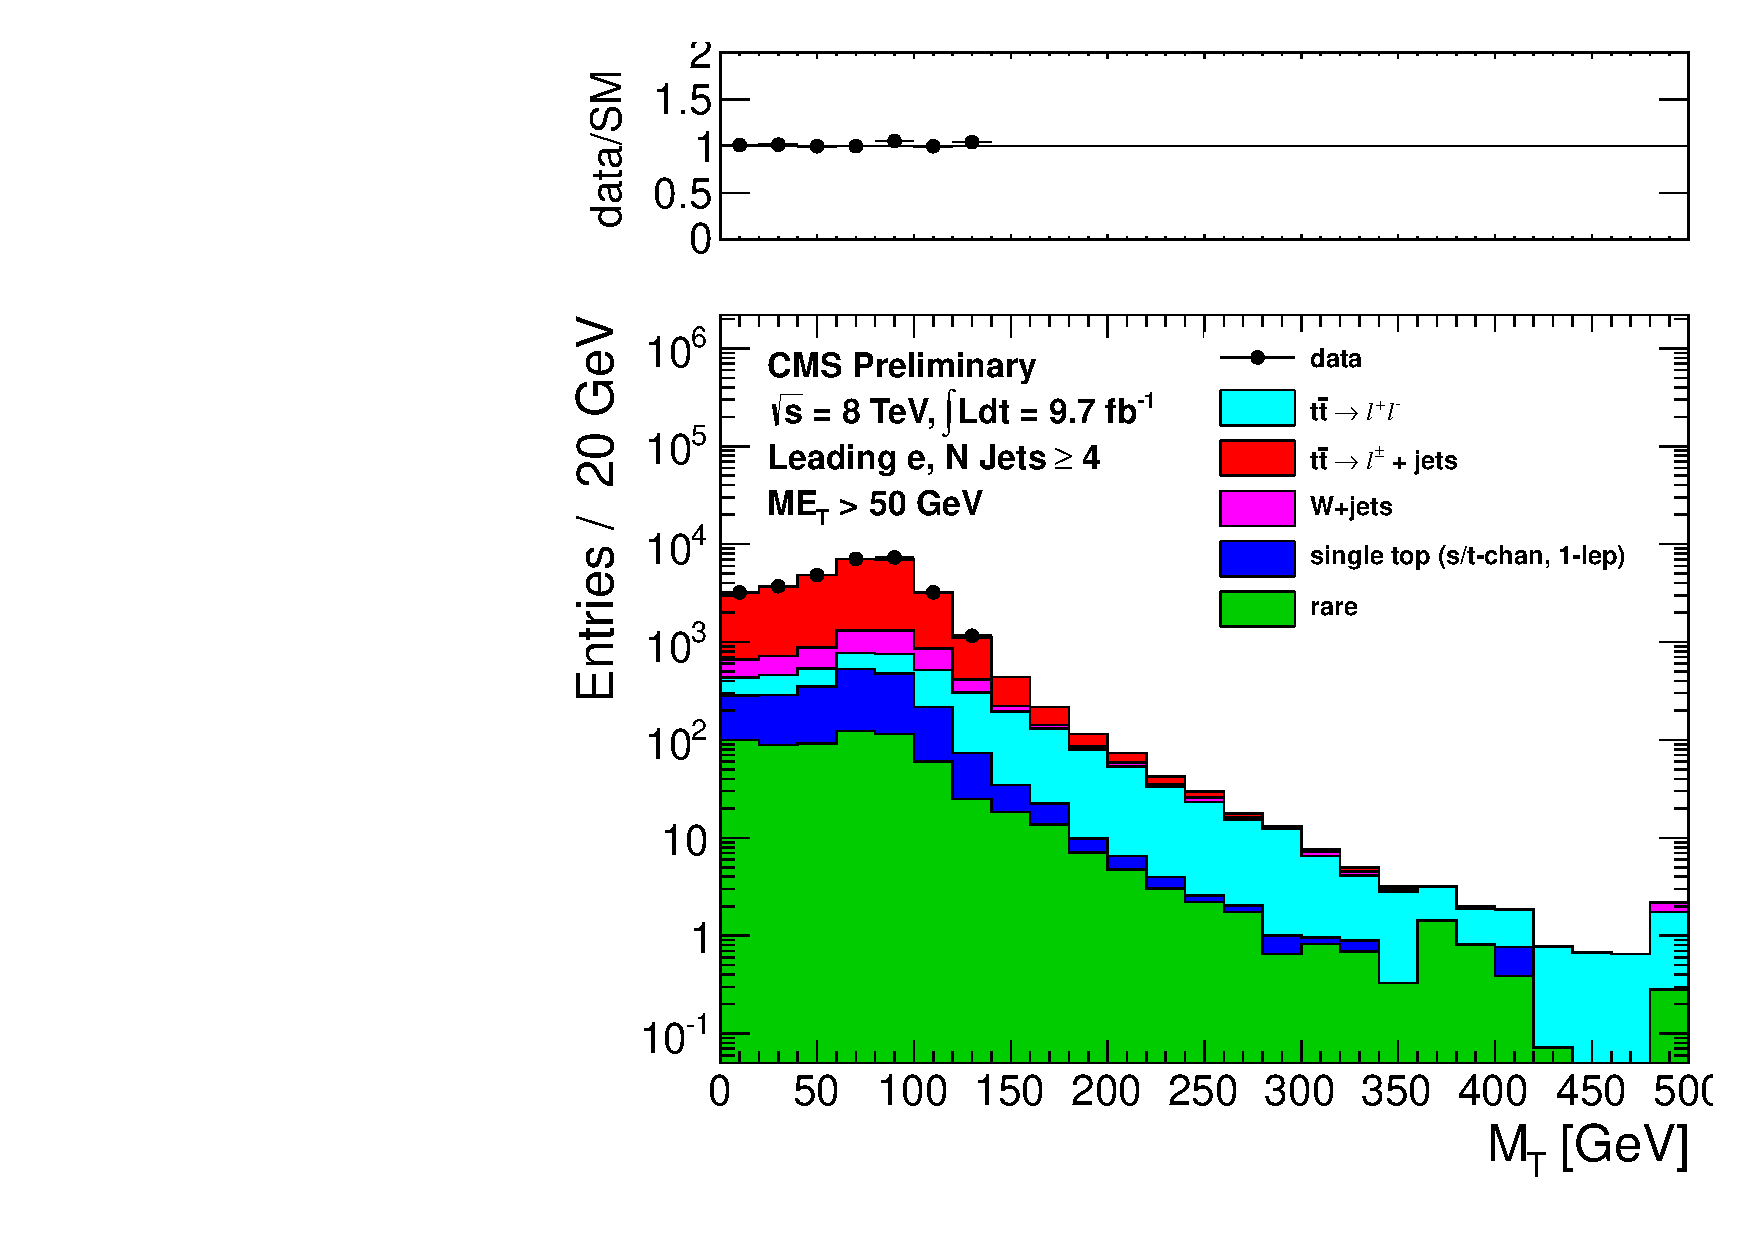
\includegraphics[width=0.5\linewidth]{plots/mt_met50_ele.pdf}%
        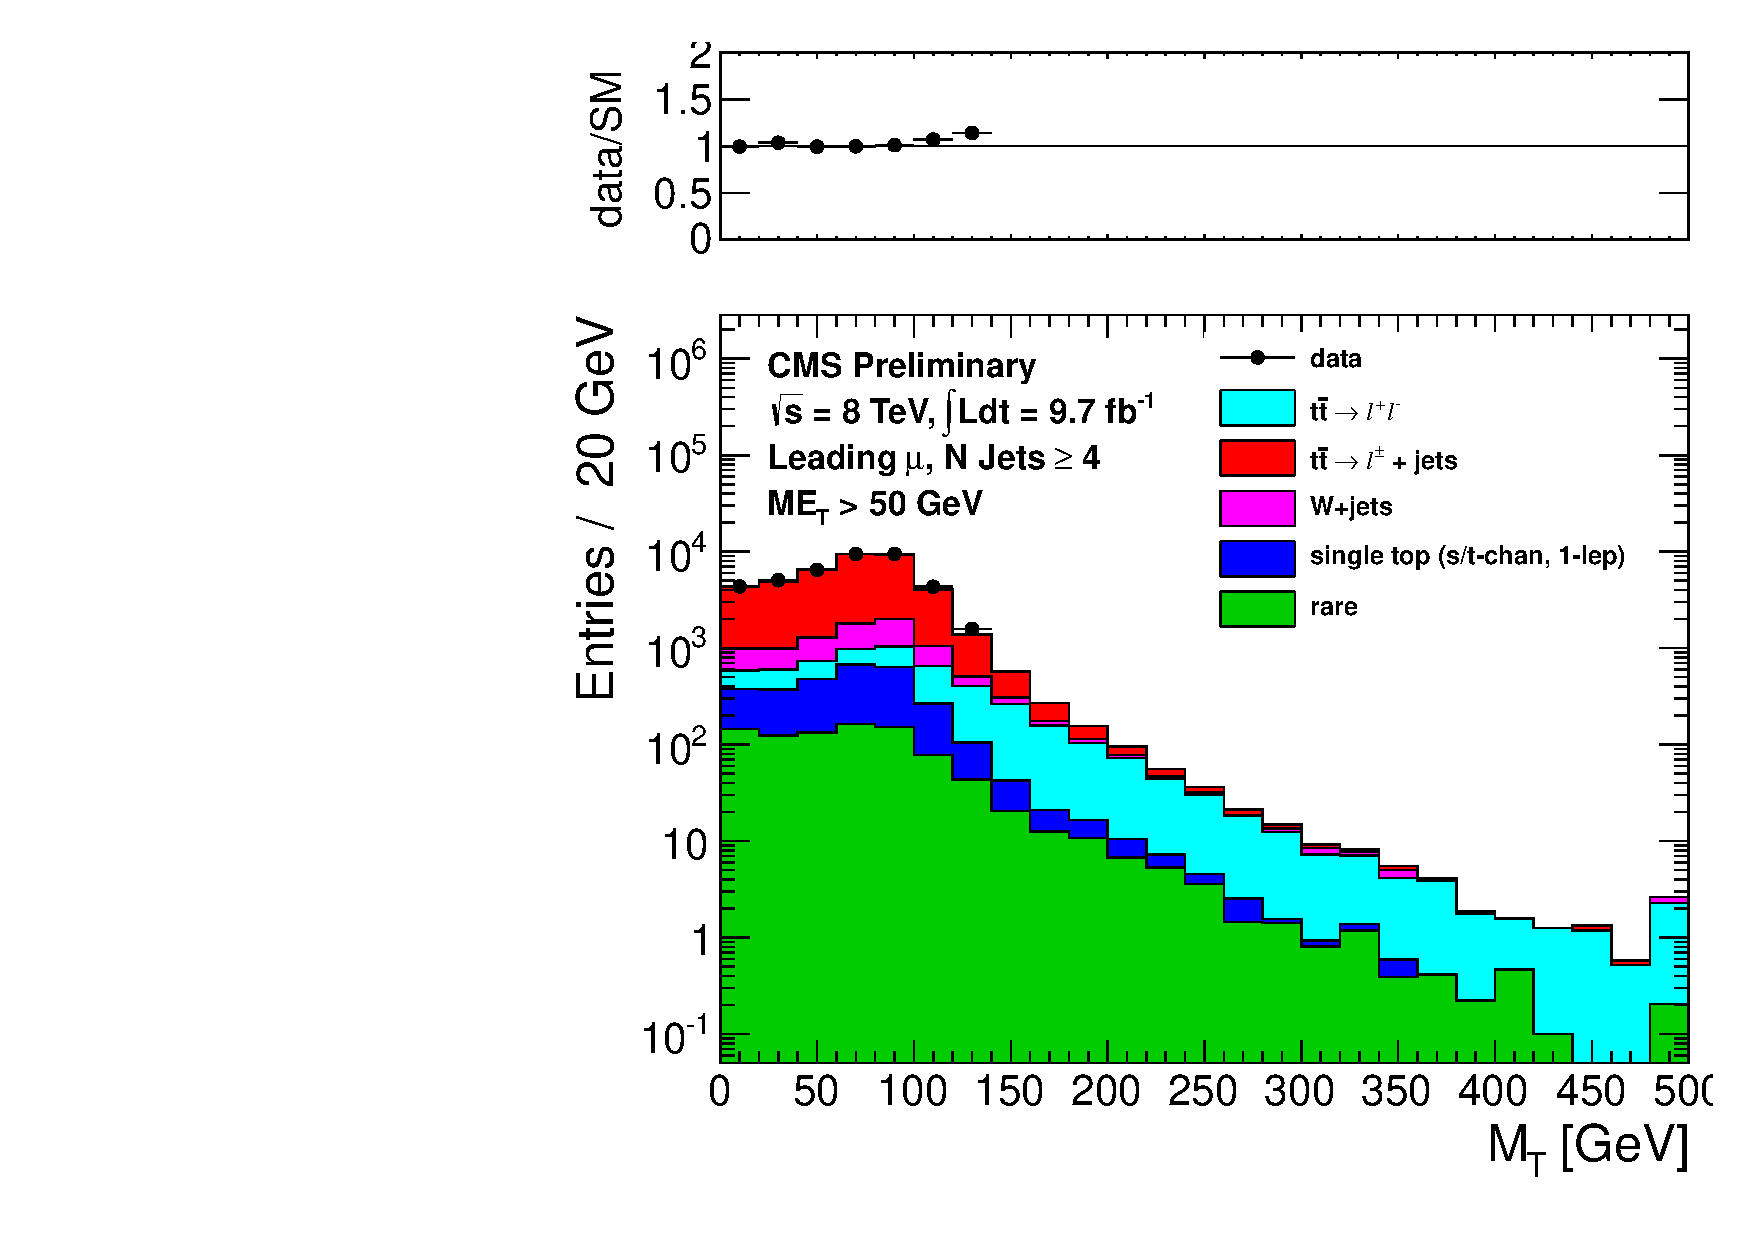
\includegraphics[width=0.5\linewidth]{plots/mt_met50_muo.pdf}
        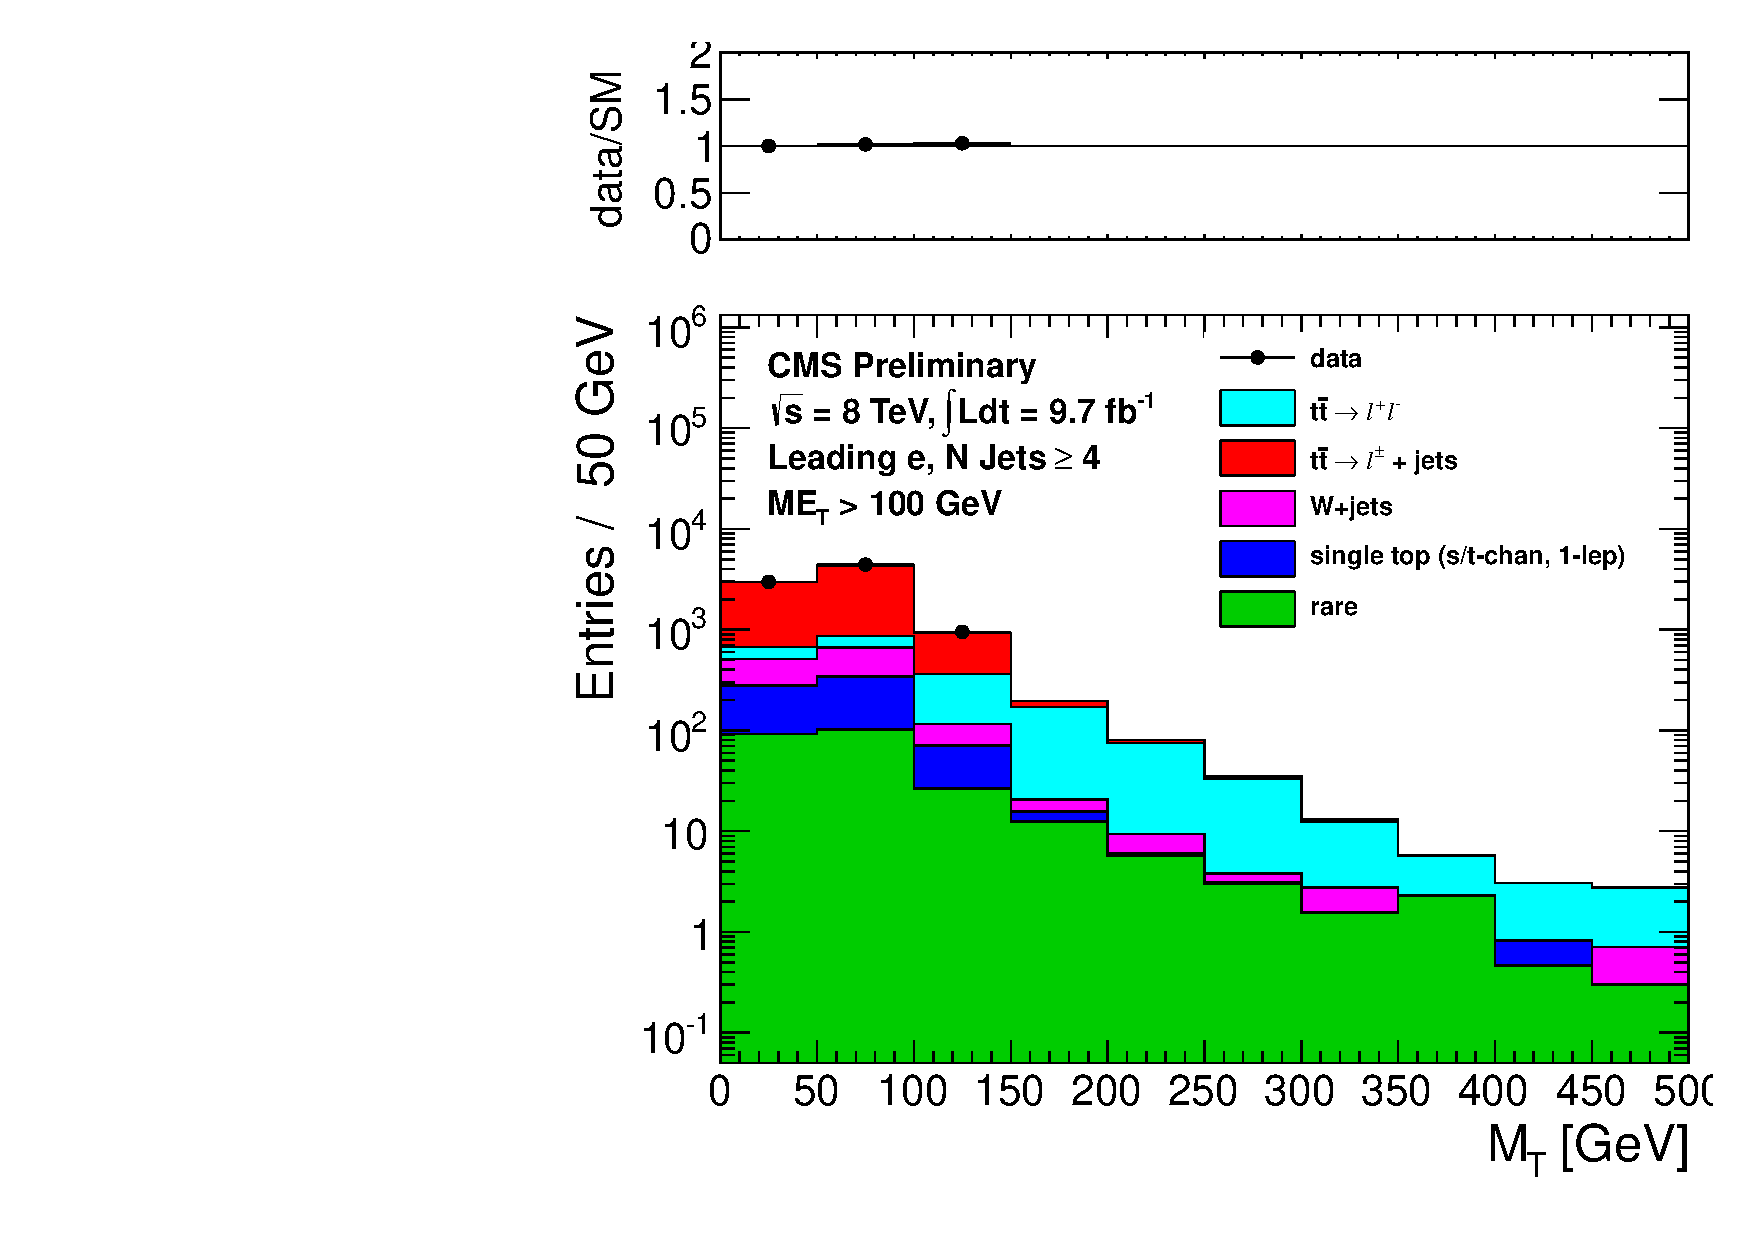
\includegraphics[width=0.5\linewidth]{plots/mt_met100_ele.pdf}%
        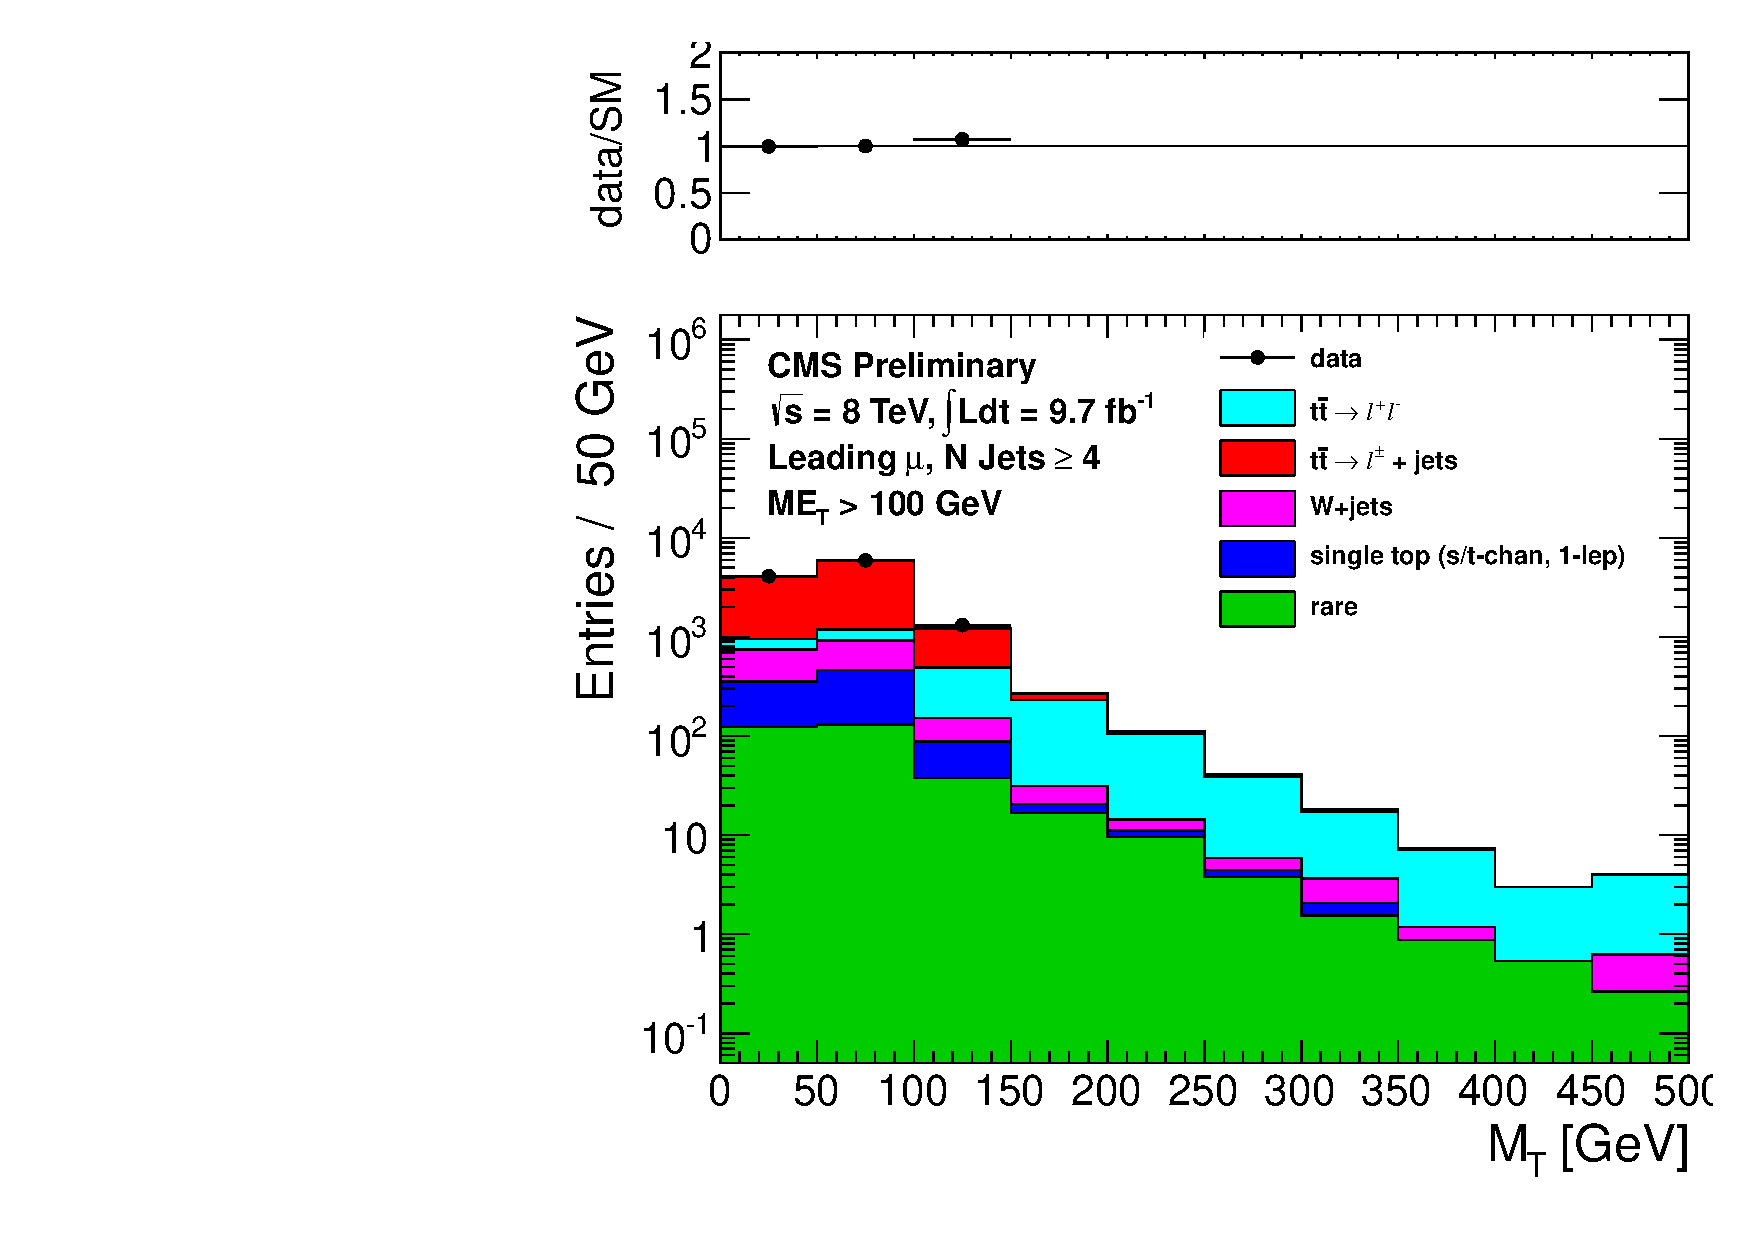
\includegraphics[width=0.5\linewidth]{plots/mt_met100_muo.pdf}
        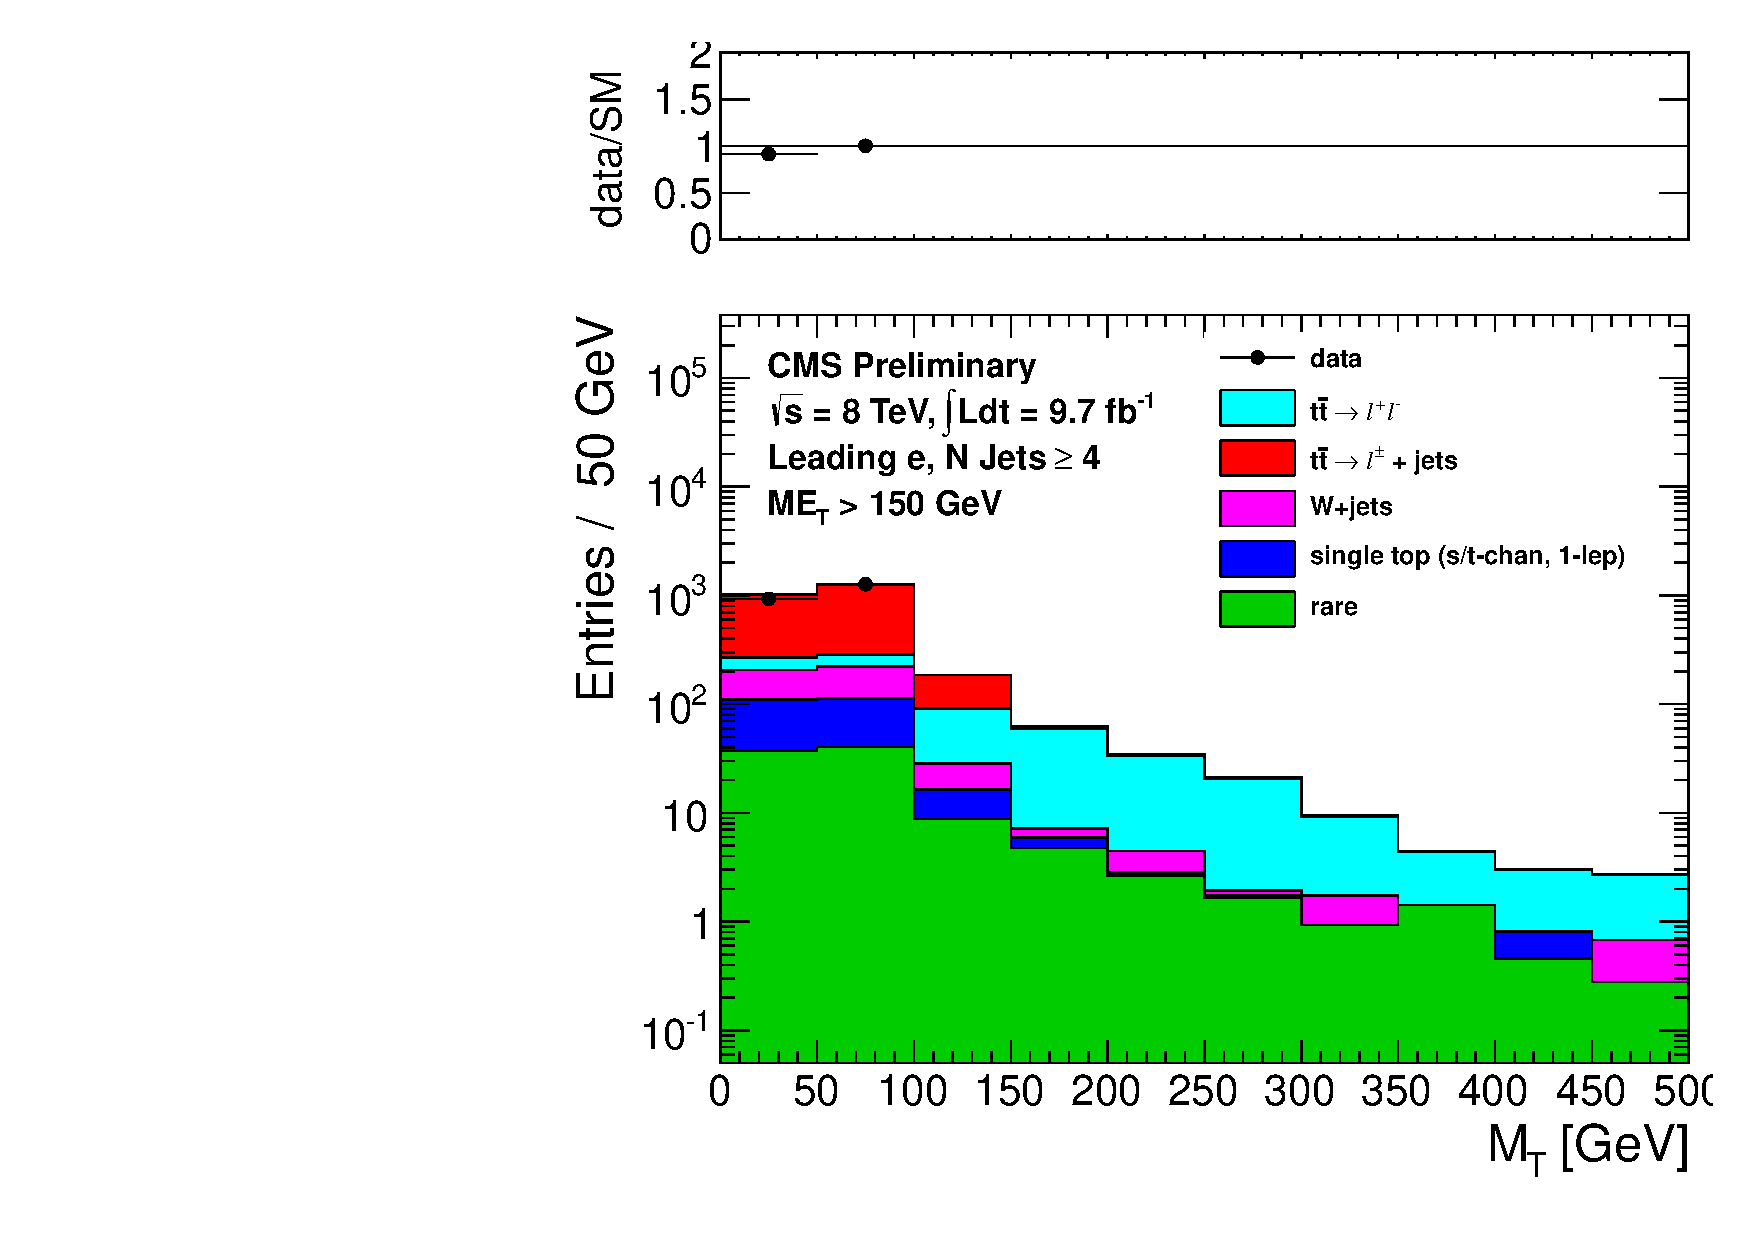
\includegraphics[width=0.5\linewidth]{plots/mt_met150_ele.pdf}%
        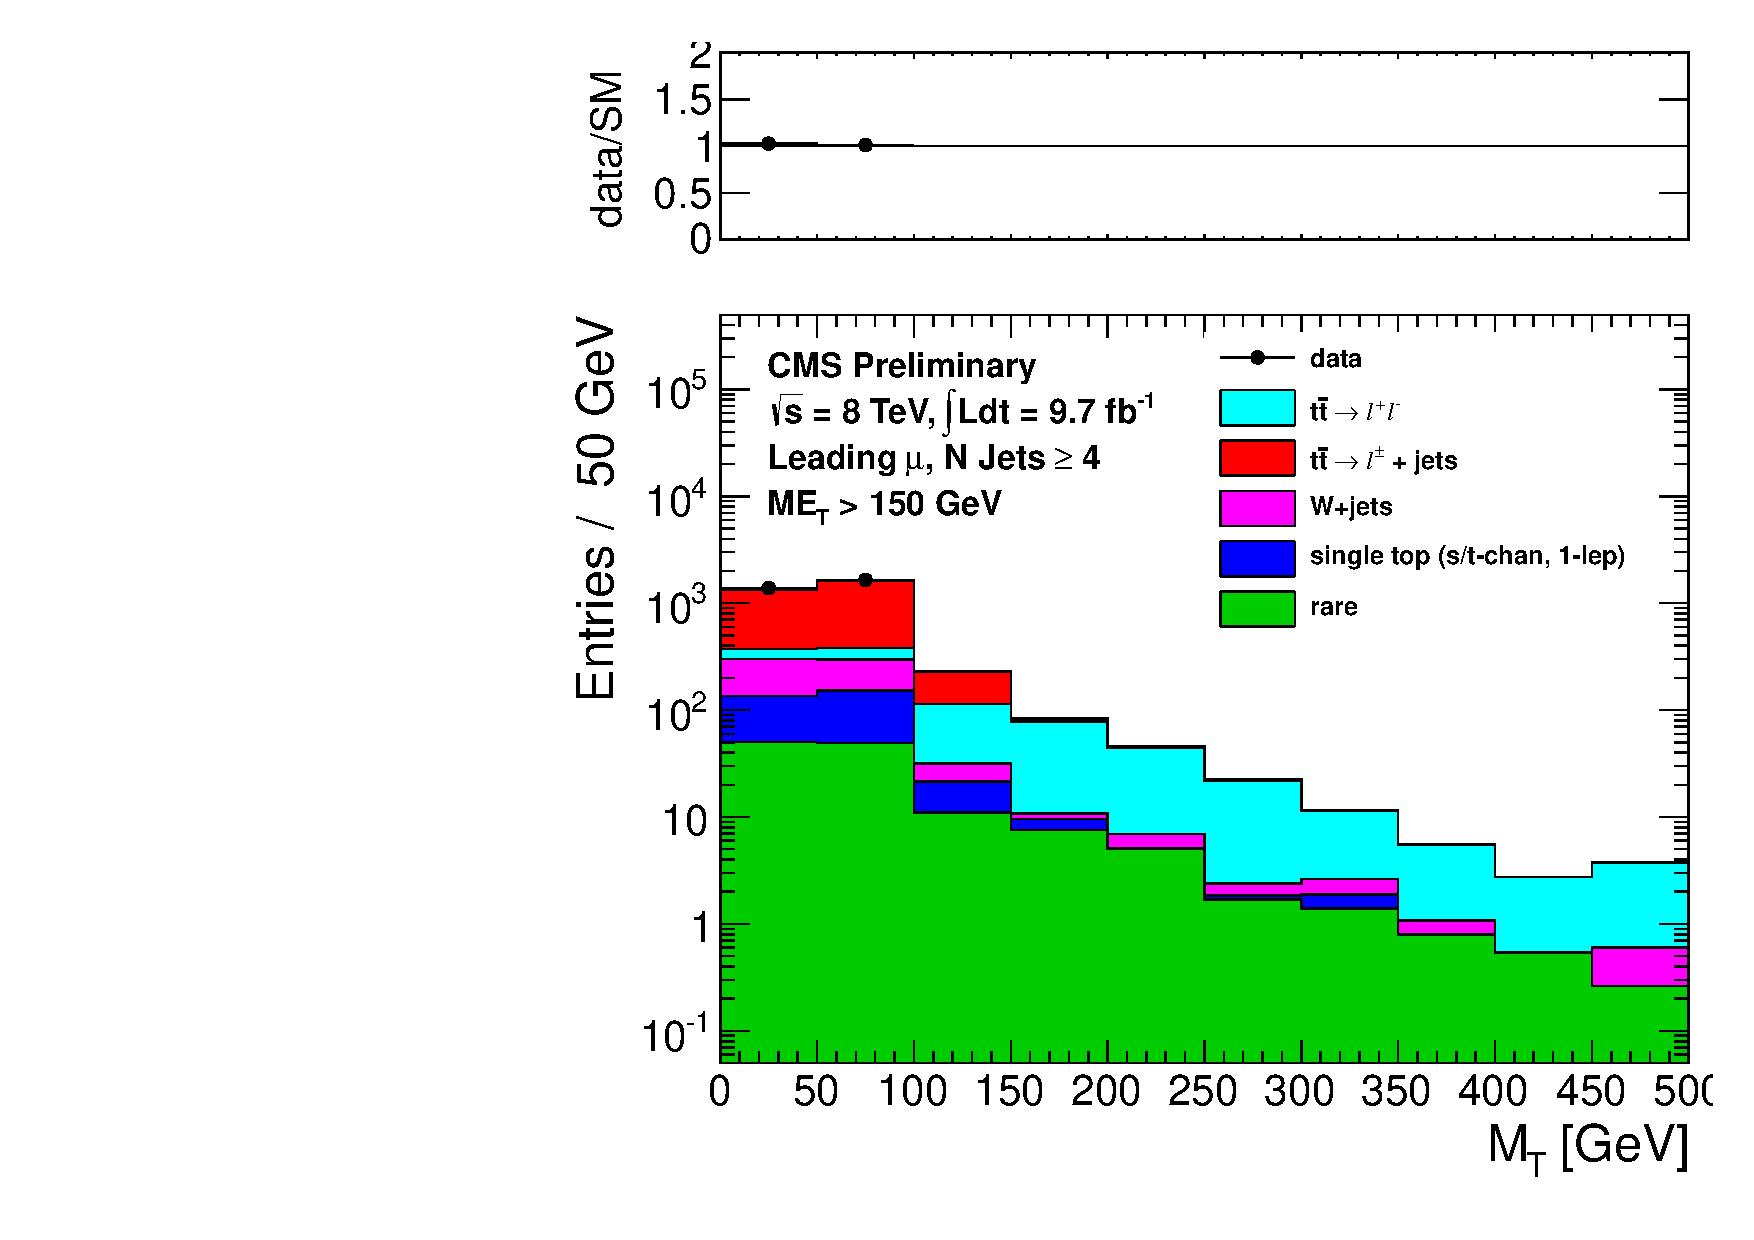
\includegraphics[width=0.5\linewidth]{plots/mt_met150_muo.pdf}

    \caption{$M_T$ in the data compared to SM Monte Carlo, for
      increasing values of \met. Note that the MC tails have not
      been rescaled at this point.
\label{fig:mtsig1}
}  
      \end{center}
\end{figure}

\begin{figure}[hbt]
  \begin{center}
        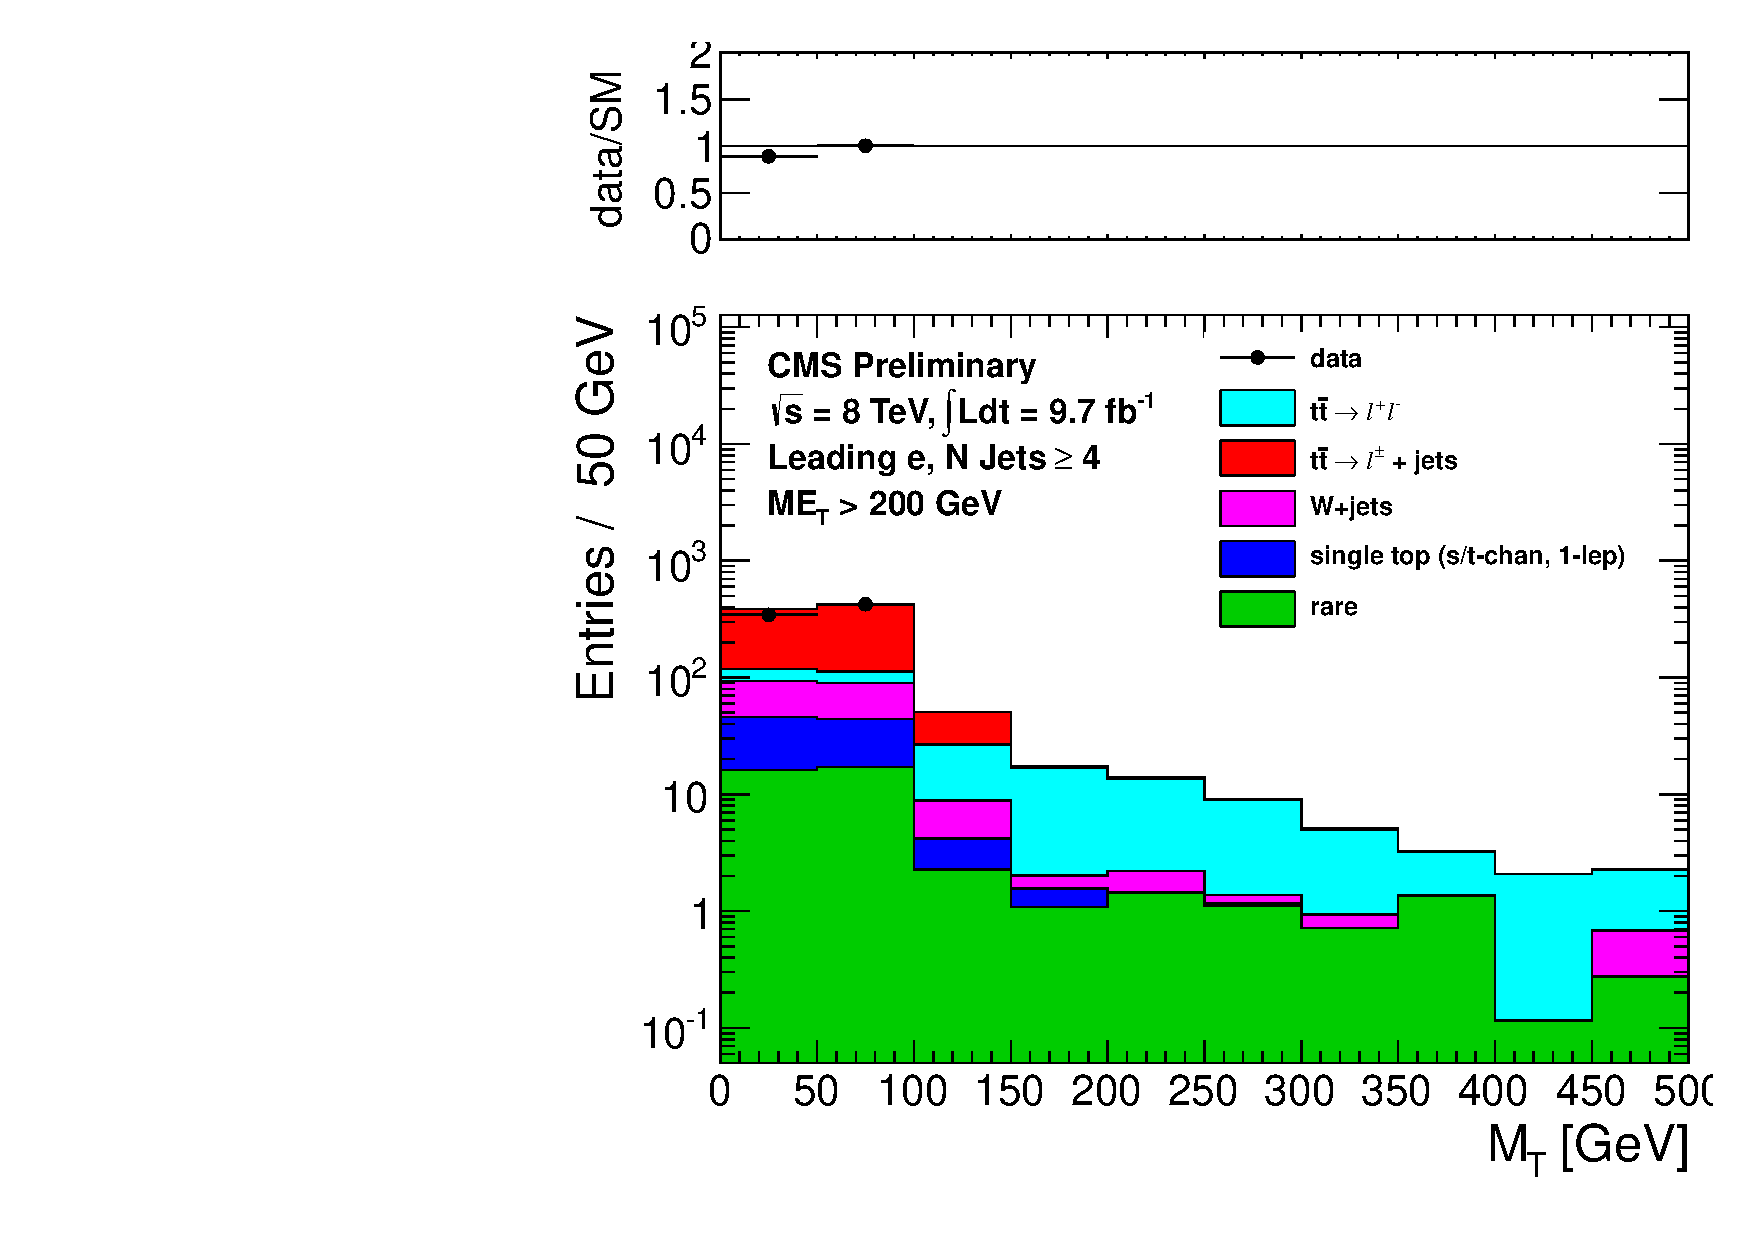
\includegraphics[width=0.5\linewidth]{plots/mt_met200_ele.pdf}%
        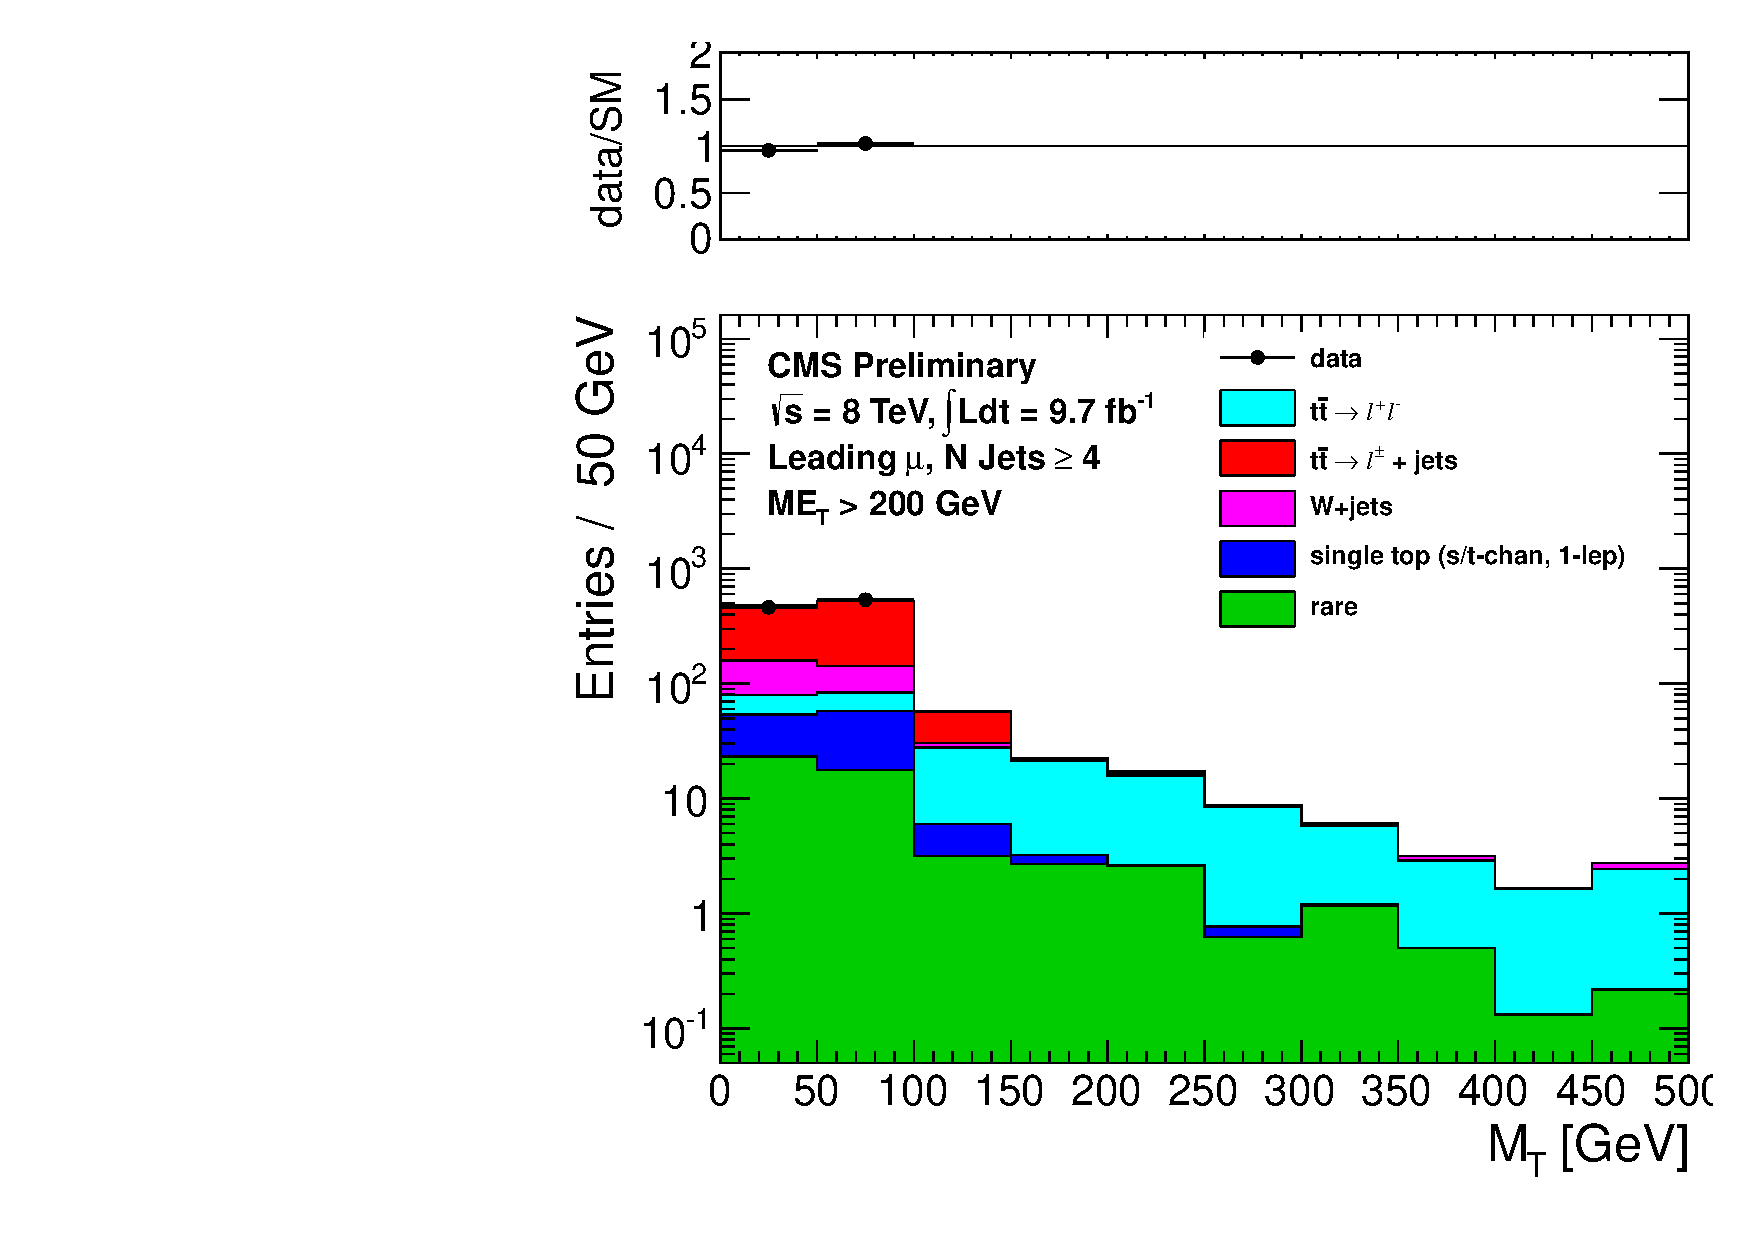
\includegraphics[width=0.5\linewidth]{plots/mt_met200_muo.pdf}
        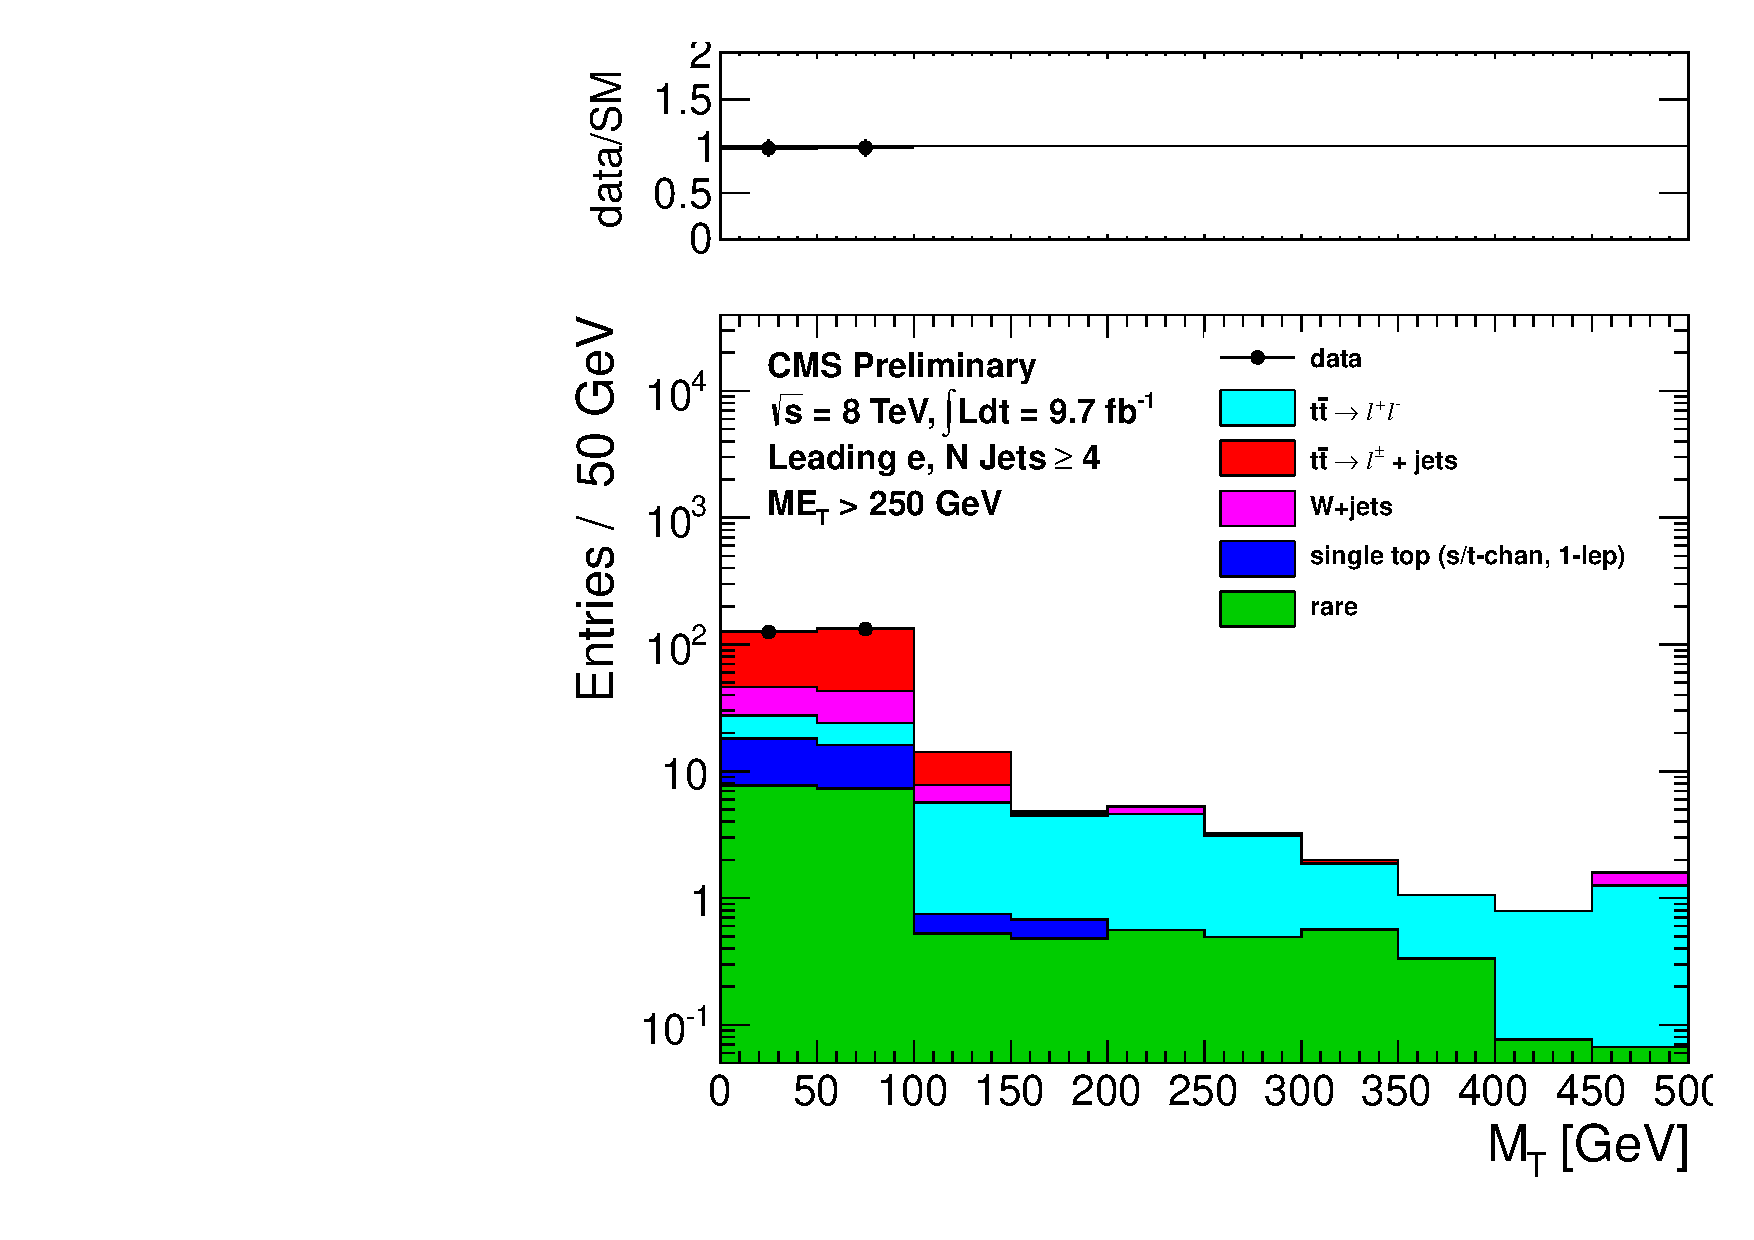
\includegraphics[width=0.5\linewidth]{plots/mt_met250_ele.pdf}%
        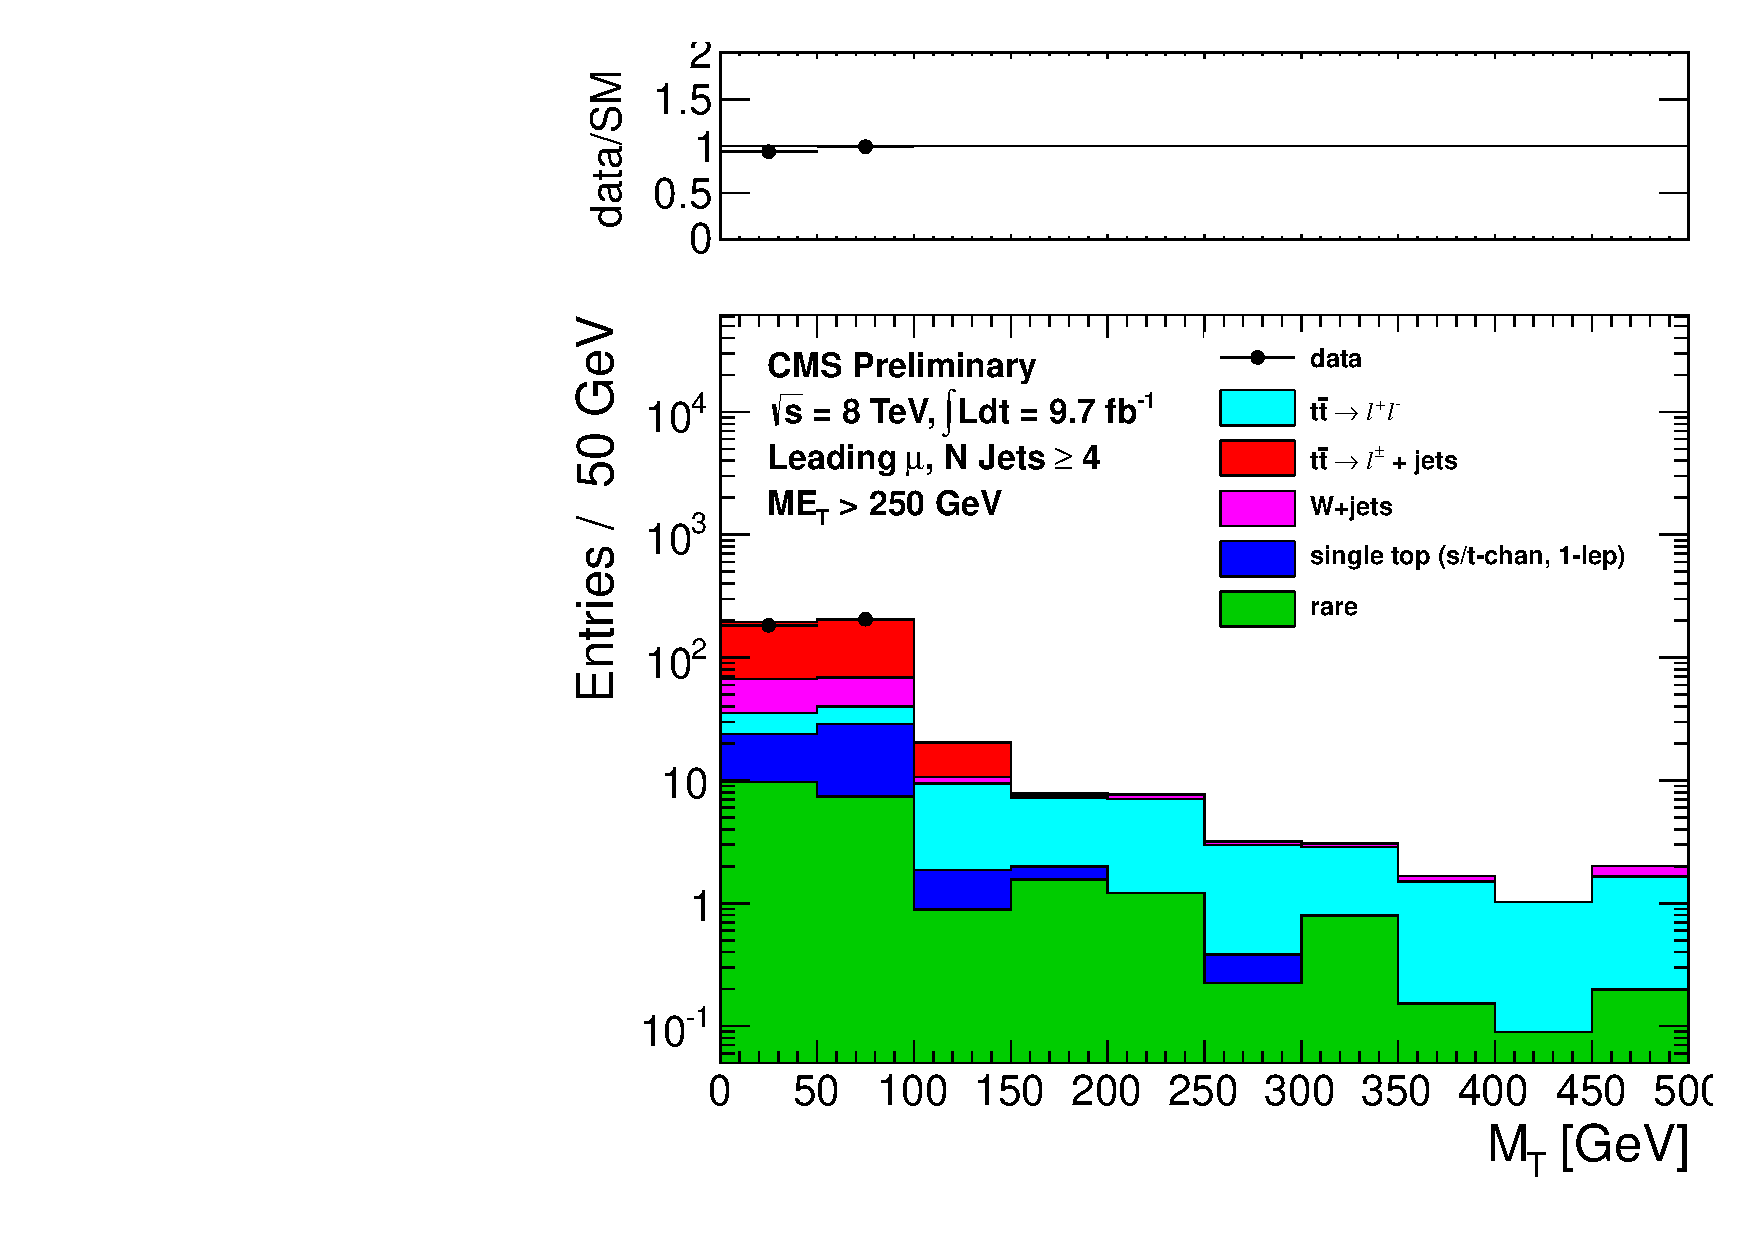
\includegraphics[width=0.5\linewidth]{plots/mt_met250_muo.pdf}
        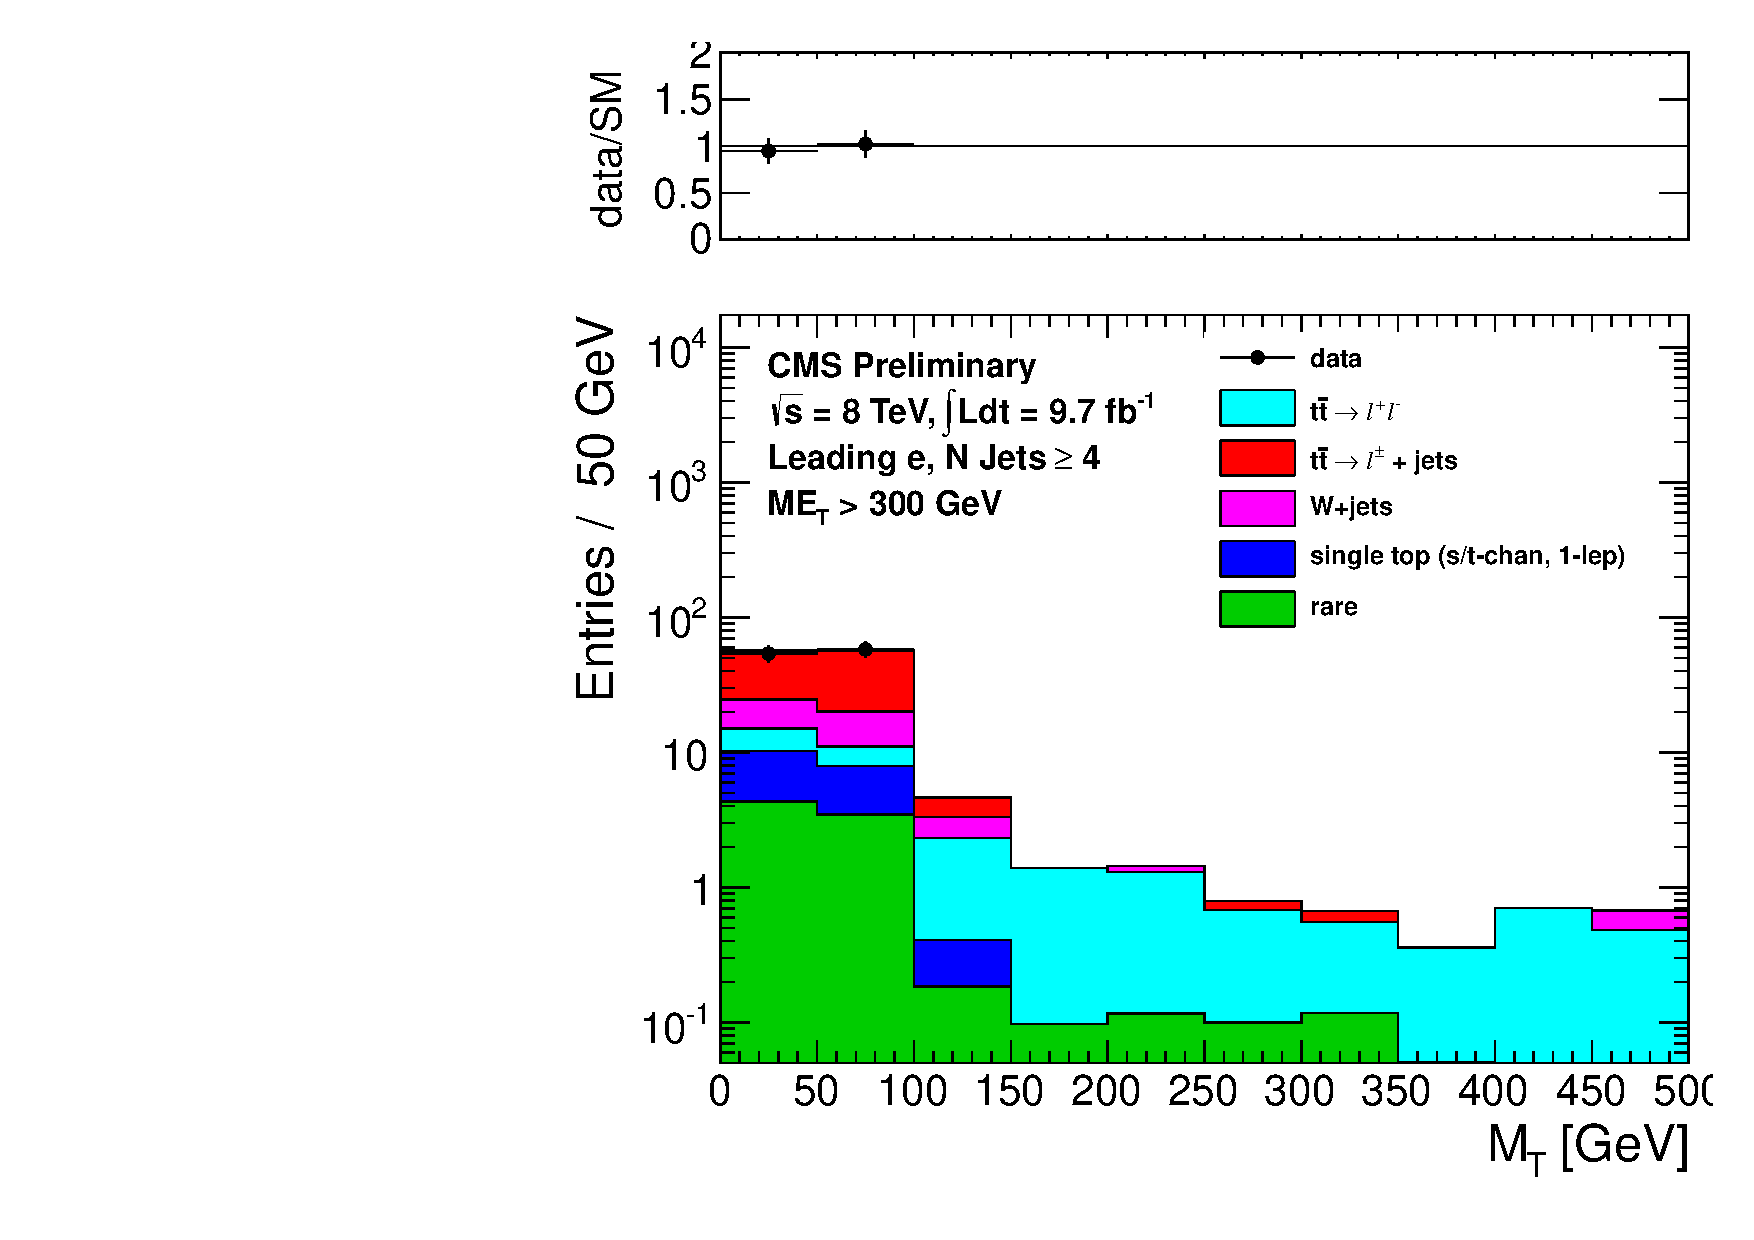
\includegraphics[width=0.5\linewidth]{plots/mt_met300_ele.pdf}%
        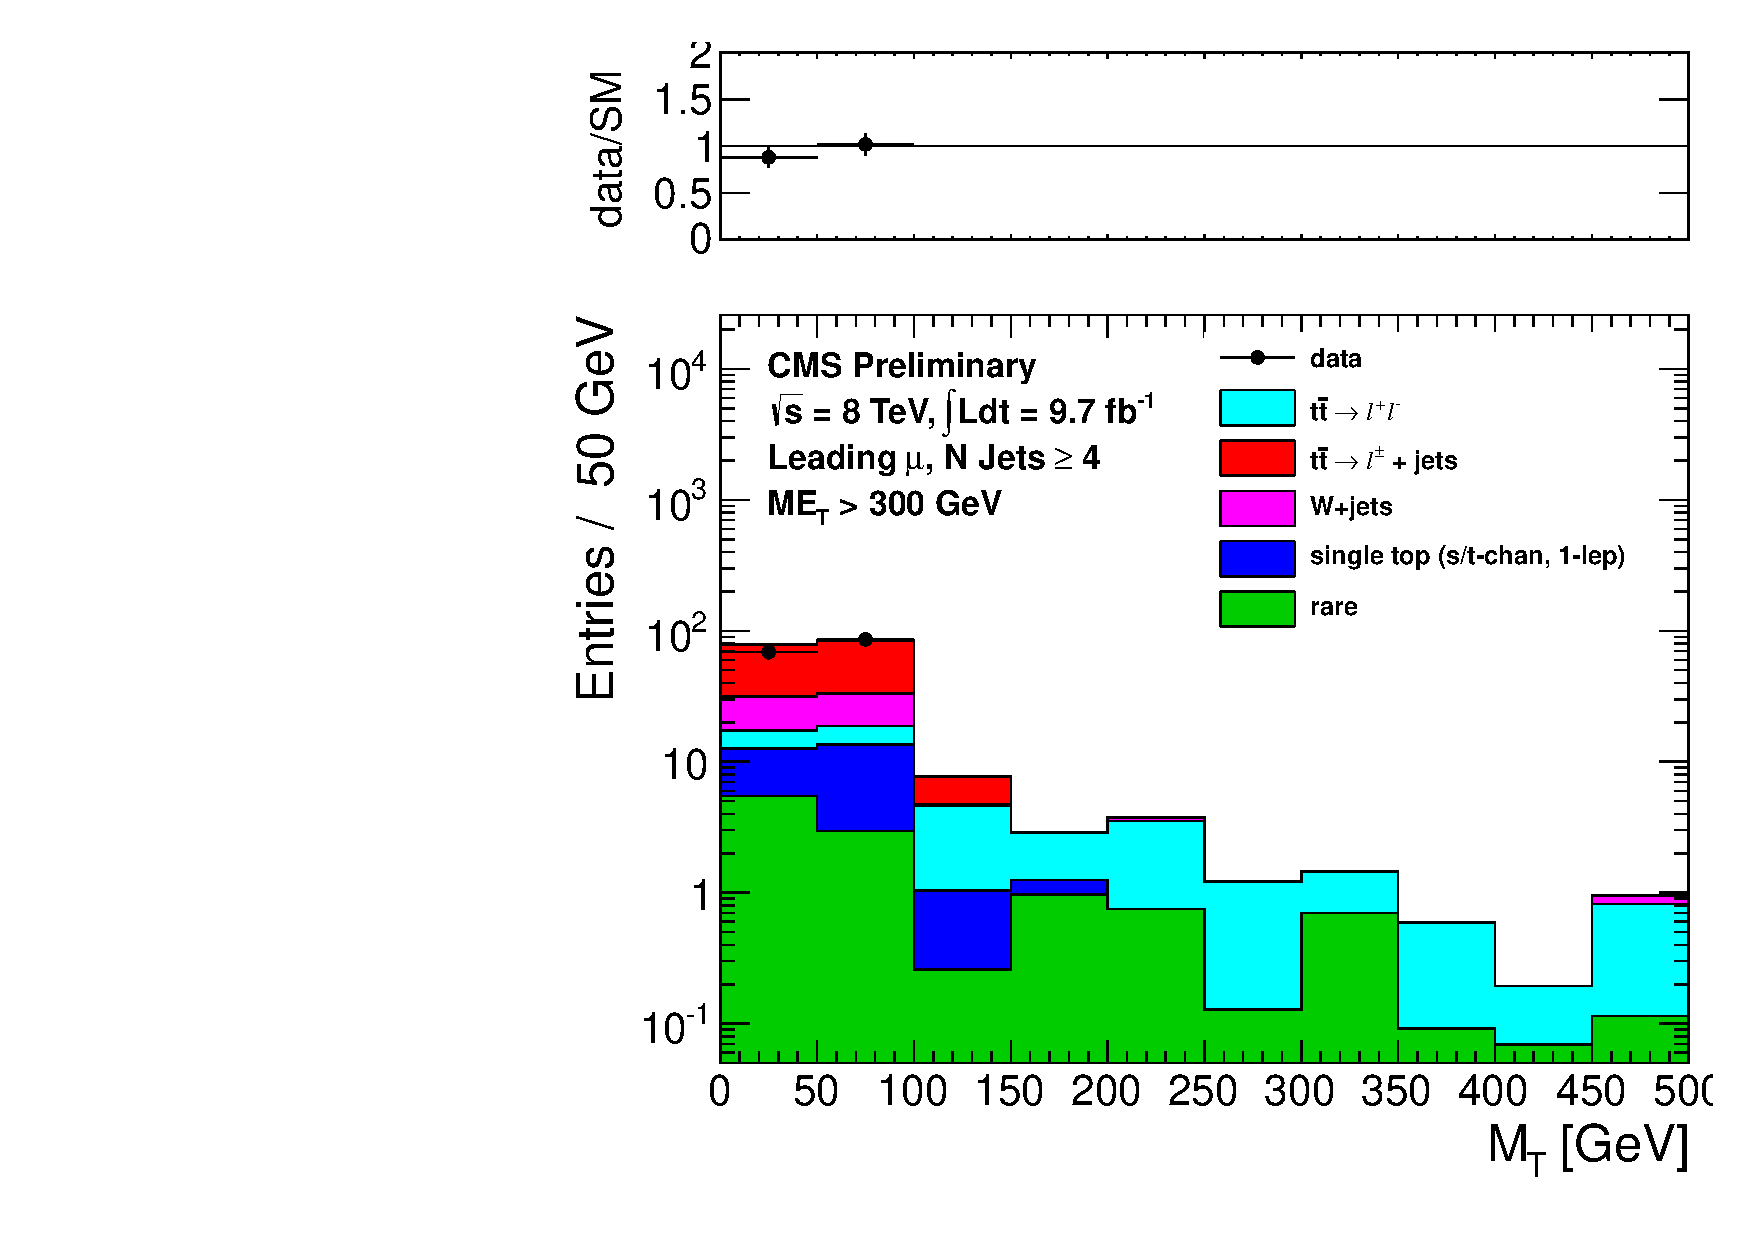
\includegraphics[width=0.5\linewidth]{plots/mt_met300_muo.pdf}

    \caption{$M_T$ in the data compared to SM Monte Carlo, for
      increasing values of \met. Note that the MC tails have not
      been rescaled at this point.
\label{fig:mtsig2}
}  
      \end{center}
\end{figure}


\begin{figure}[hbt]
  \begin{center}
        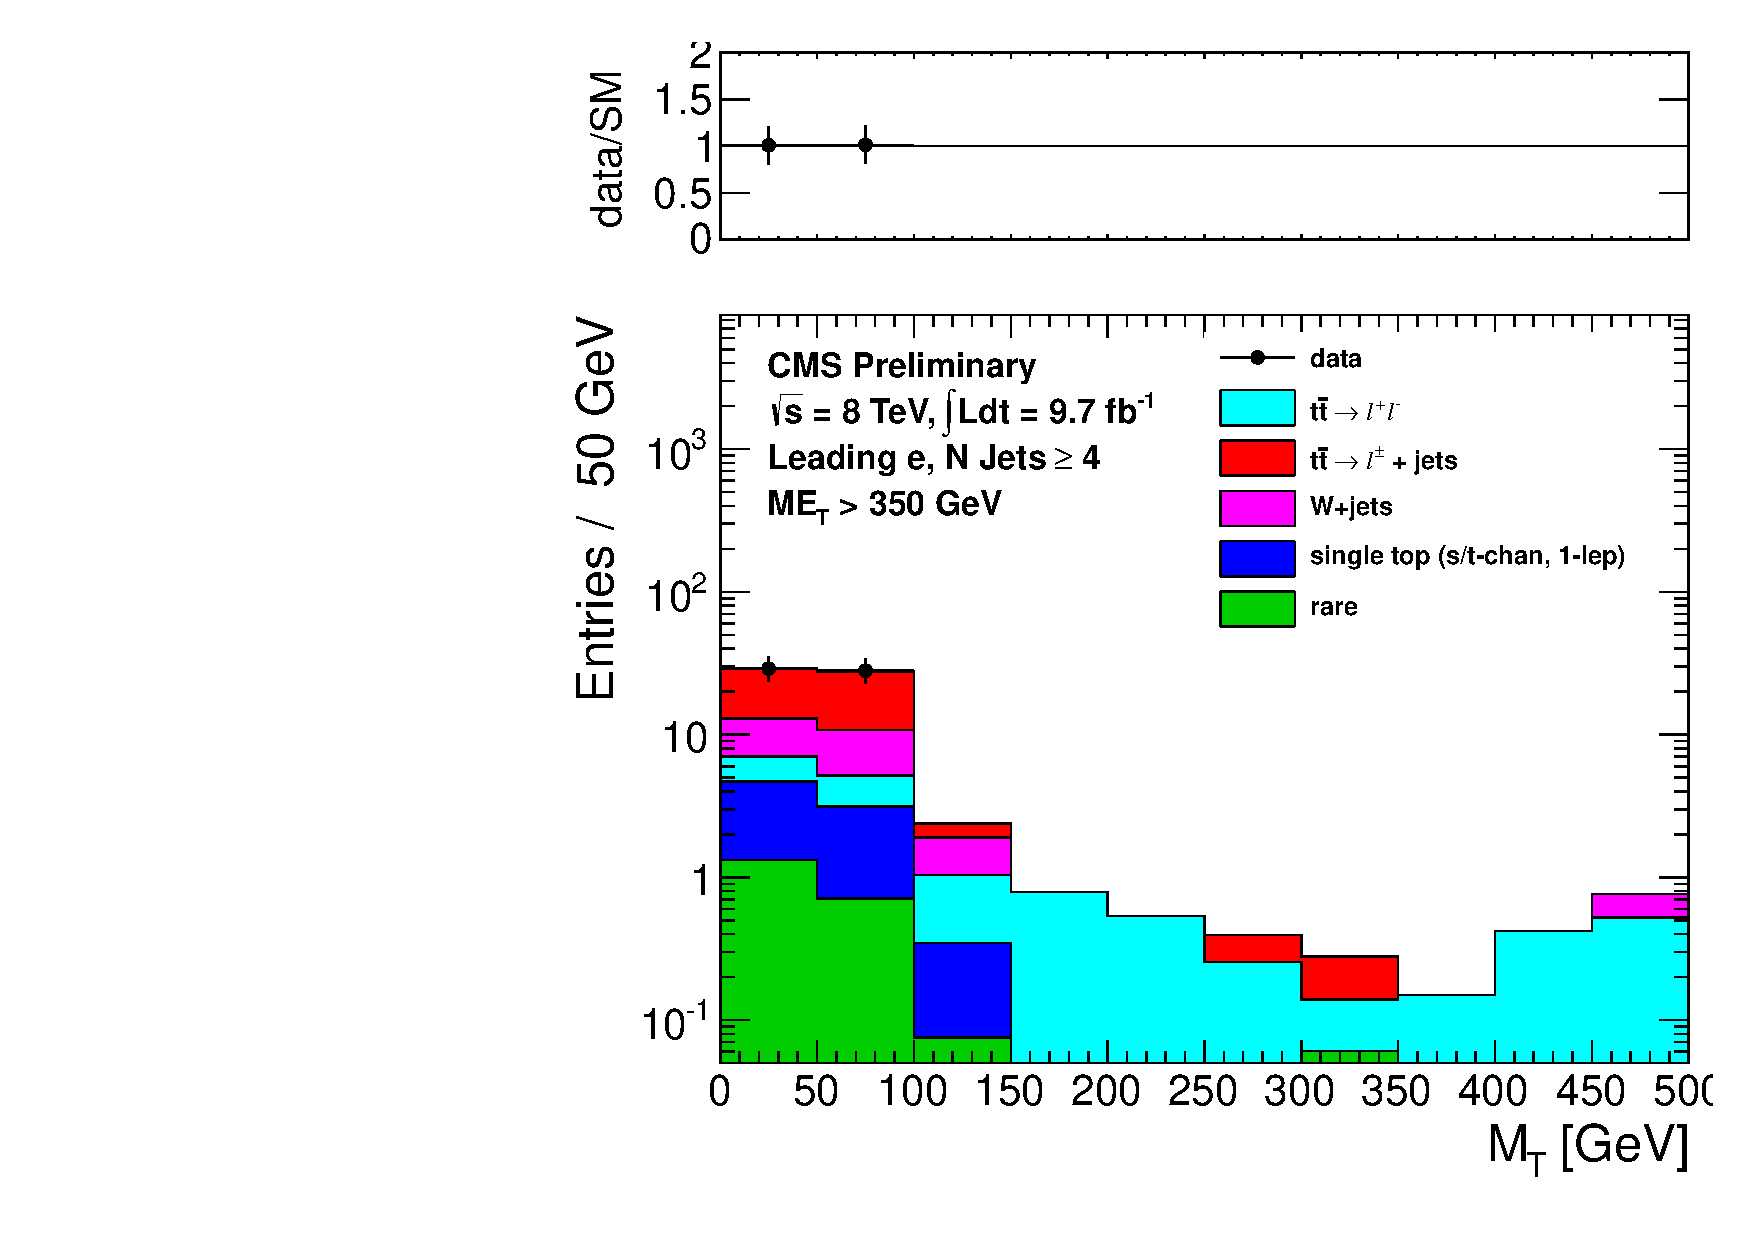
\includegraphics[width=0.5\linewidth]{plots/mt_met350_ele.pdf}%
        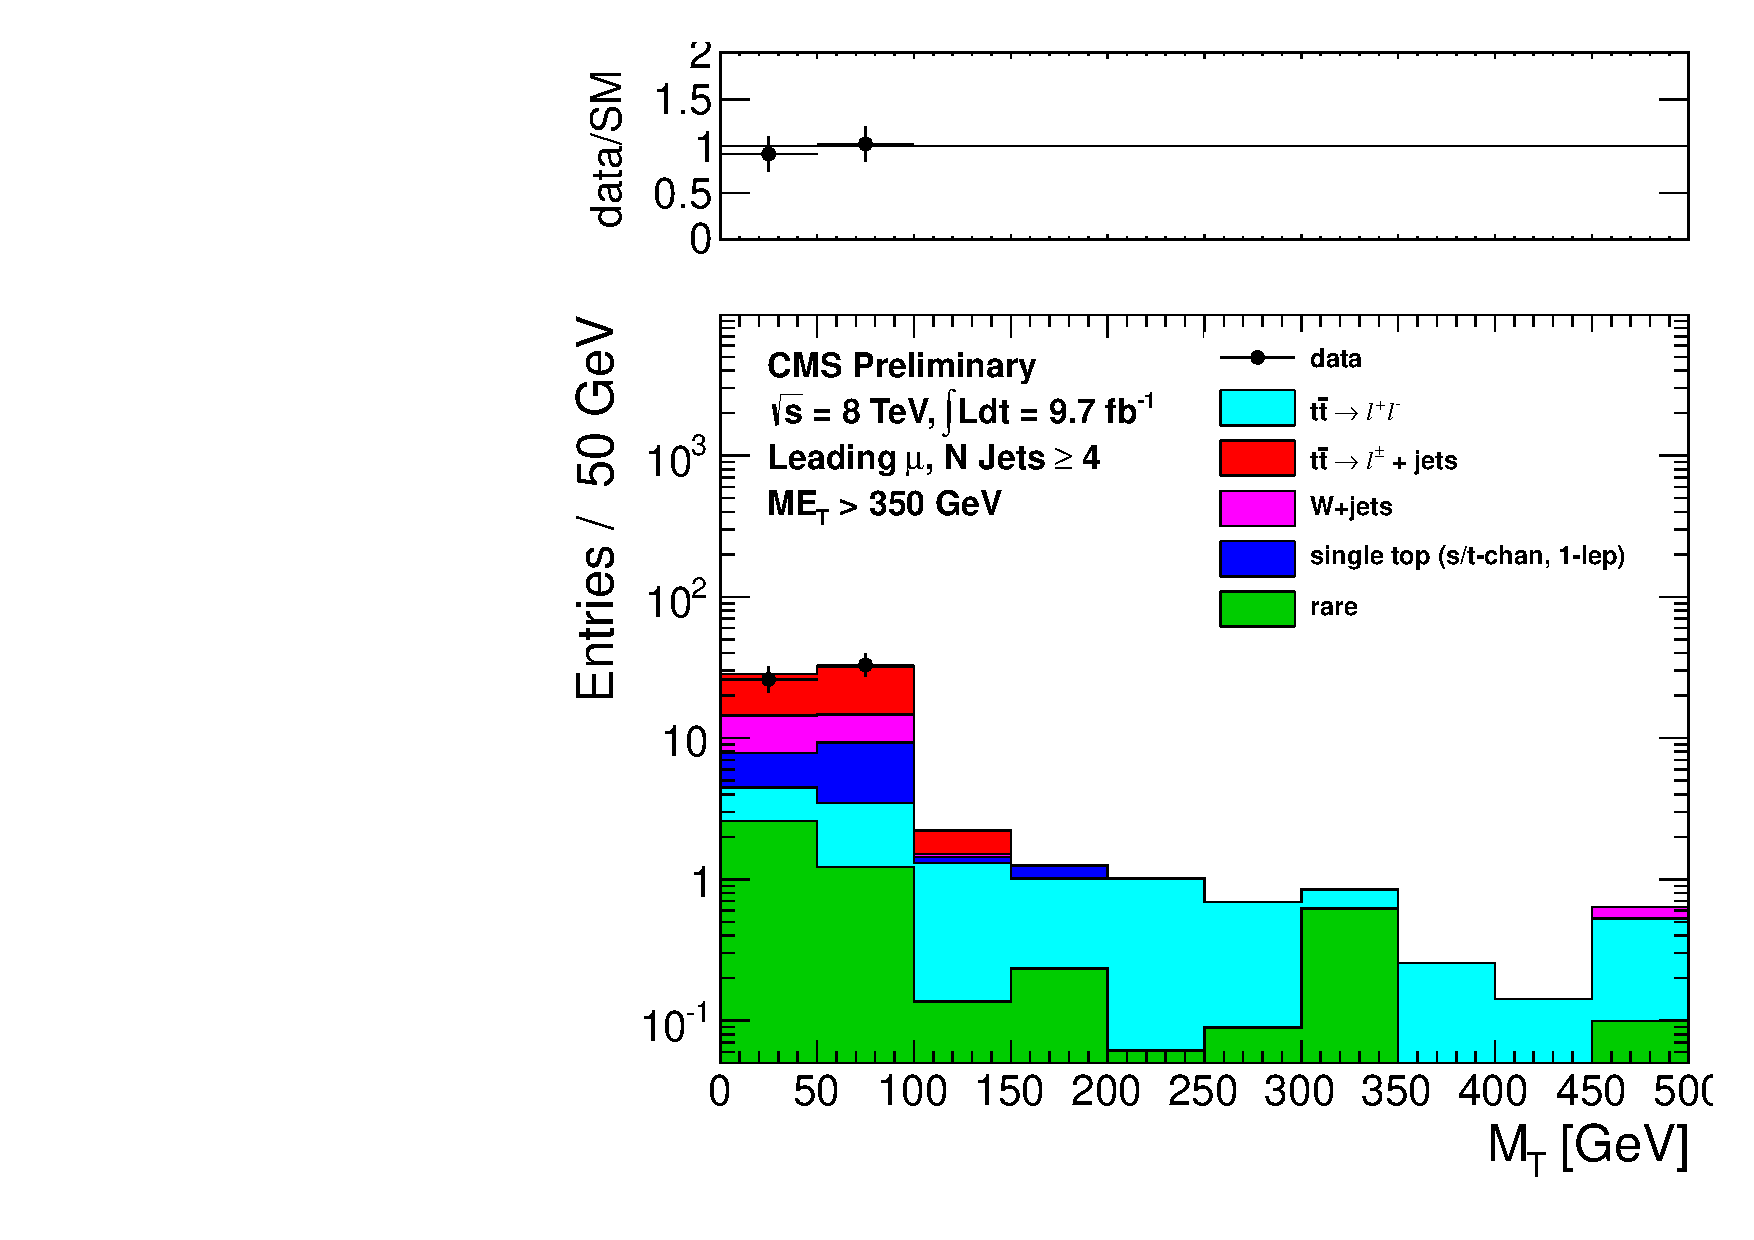
\includegraphics[width=0.5\linewidth]{plots/mt_met350_muo.pdf}
        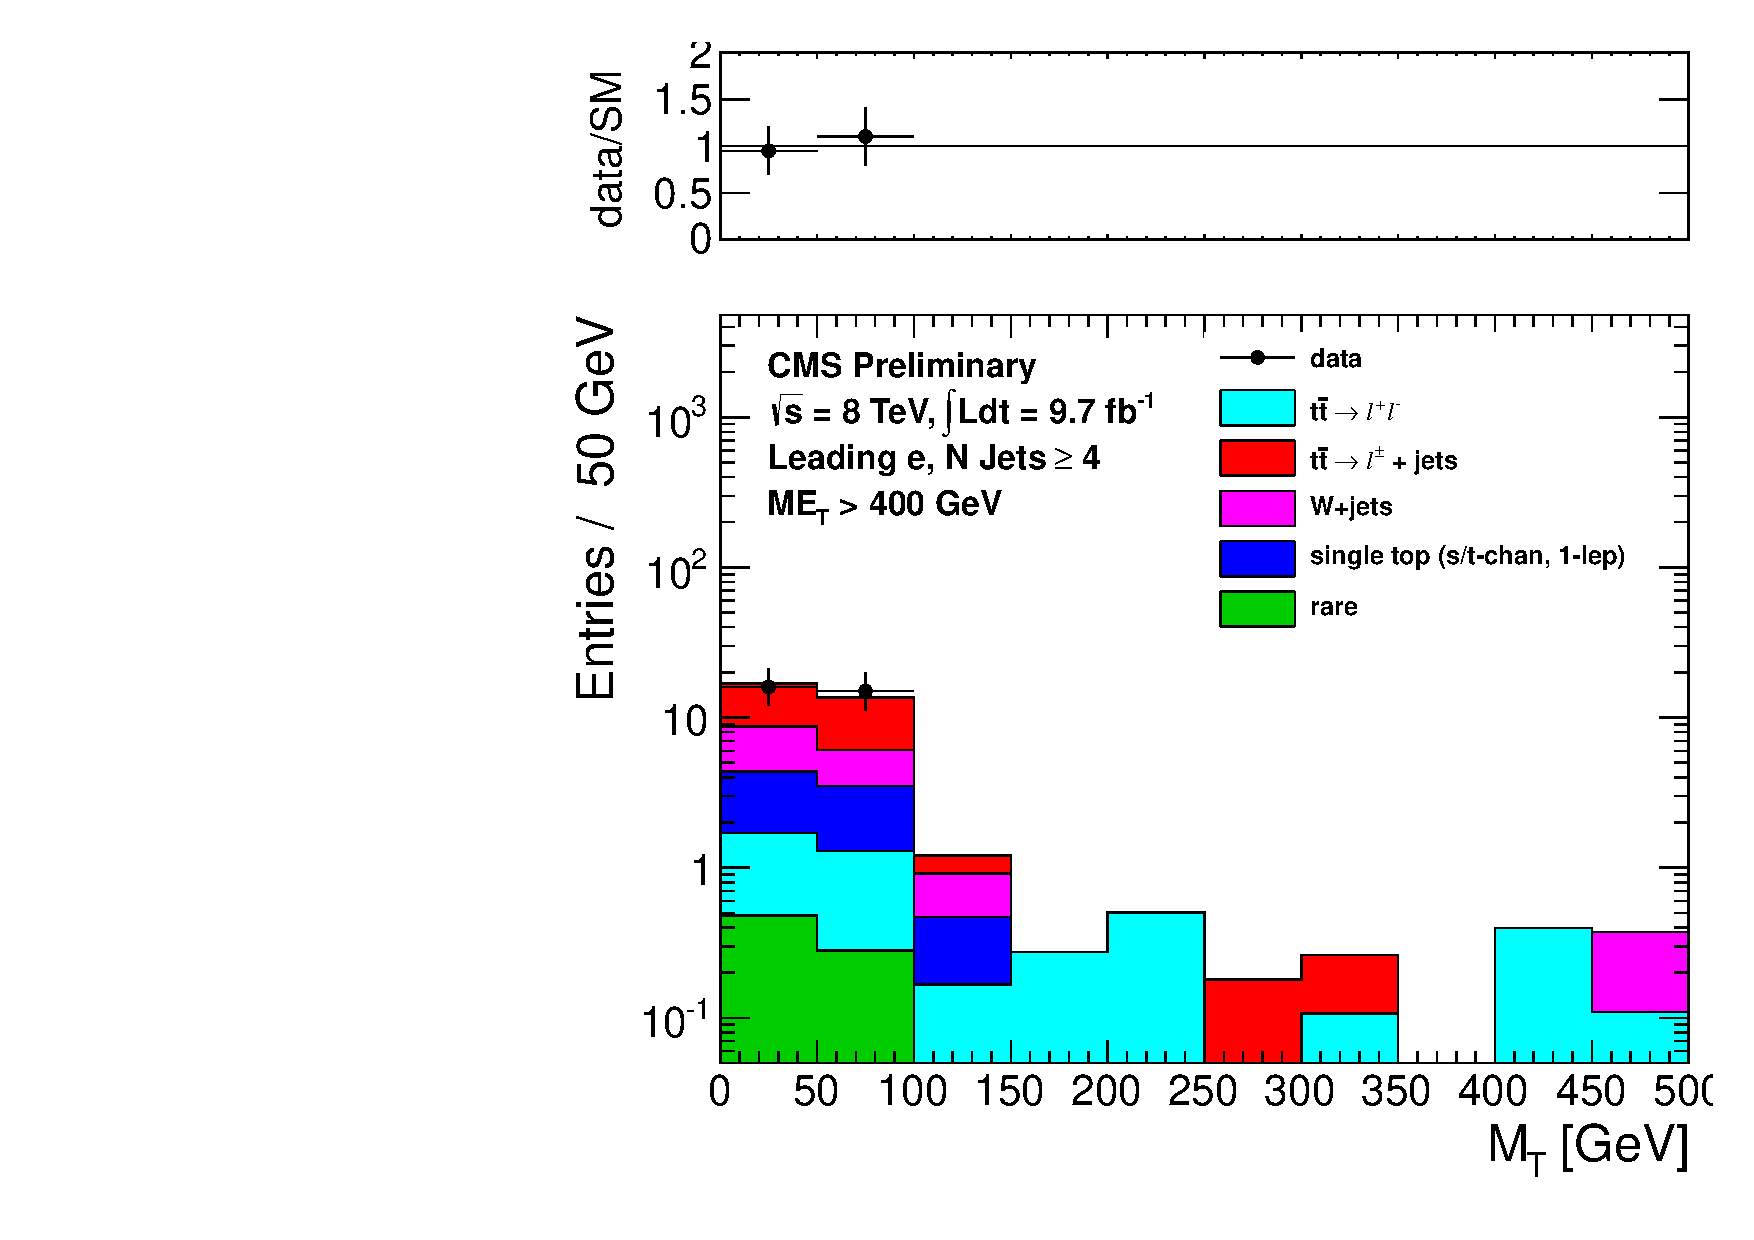
\includegraphics[width=0.5\linewidth]{plots/mt_met400_ele.pdf}%
        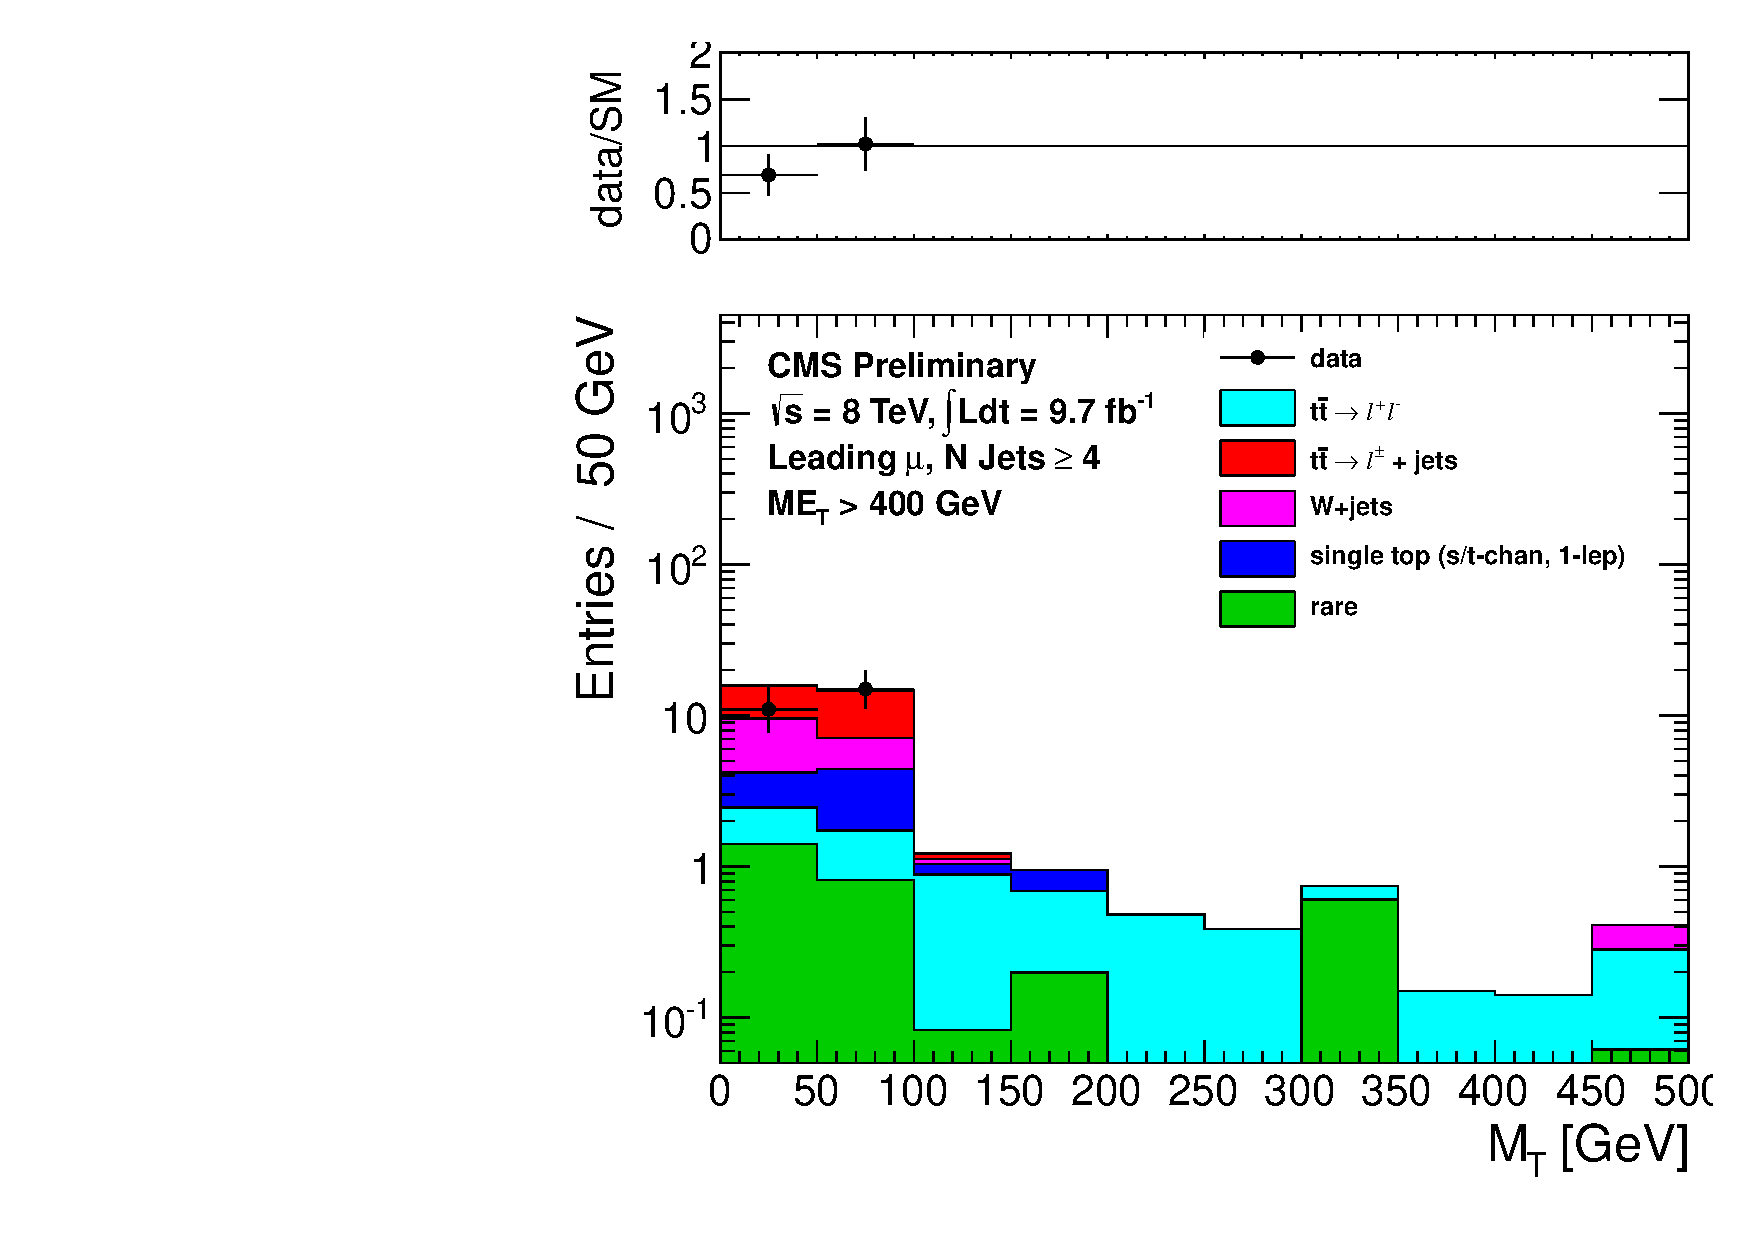
\includegraphics[width=0.5\linewidth]{plots/mt_met400_muo.pdf}

    \caption{$M_T$ in the data compared to SM Monte Carlo, for
      increasing values of \met. Note that the MC tails have not
      been rescaled at this point.
\label{fig:mtsig3}
}  
      \end{center}
\end{figure}

\clearpage
